\documentclass[a4paper]{article}
\usepackage[utf8]{inputenc}
\usepackage[T1]{fontenc}
\usepackage{aeguill}
\usepackage{hyperref}
\usepackage{verbatim}
\usepackage{amsmath}
\usepackage{amsfonts}
\usepackage{tikz}
\usepackage{a4wide}



\newcommand{\strid}{\textsl{strid}}
\newcommand{\example}[1]{\begin{center}\fbox{\begin{minipage}{11cm}#1\end{minipage}}\end{center}}
\newcommand{\cinput}[1]{\vcenter{\hbox{\input{#1}}}}

\title{strid -- A string diagrams generator}
\author{Samuel Mimram}
\begin{document}
\maketitle
\tableofcontents
\newpage

\strid{} is a string diagrams generator for inclusion into \LaTeX{} files. It is
still in very $\alpha$ stage but already quite useable. It is entirely
programmed in OCaml\footnote{OCaml can be downloaded at
  \url{http://caml.inria.fr/}.}. Feel free to drop me a line at
\url{samuel.mimram@pps.jussieu.fr} if you have some comments, bug reports or
feature requests about it.

\section{Presentation of \strid{}}
\subsection{A first example}
%\begin{figure}[ht!]
\example{ Suppose that $(\mathcal{C},\otimes,I)$ is a strict monoidal
  category. A \emph{monoid} in $\mathcal{C}$ is an object $M$ of $\mathcal{C}$
  together with two maps $\mu:M\otimes M\to M$, called \emph{multiplication},
  and $\eta:I\to M$, called \emph{unit}, respectively drawn as
\[
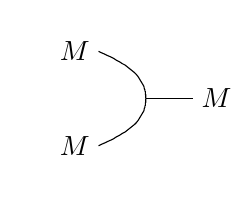
\begin{tikzpicture}[scale=0.60]
\useasboundingbox (-0.5,-0.5) rectangle (3.5,2.5);
\draw (2.00,1.00) -- (3.00,1.00);
\draw (1.00,2.00) -- (1.06,1.97) -- (1.13,1.94) -- (1.19,1.91) -- (1.26,1.88) -- (1.32,1.85) -- (1.38,1.81) -- (1.44,1.78) -- (1.50,1.74) -- (1.56,1.71) -- (1.61,1.67) -- (1.66,1.63) -- (1.71,1.59) -- (1.76,1.55) -- (1.80,1.51) -- (1.84,1.46) -- (1.87,1.41) -- (1.90,1.36) -- (1.93,1.31) -- (1.96,1.26) -- (1.97,1.20);
\draw (1.97,1.20) -- (1.98,1.19) -- (1.98,1.18) -- (1.98,1.17) -- (1.98,1.16) -- (1.99,1.15) -- (1.99,1.14) -- (1.99,1.13) -- (1.99,1.12) -- (1.99,1.11) -- (1.99,1.10) -- (1.99,1.09) -- (2.00,1.08) -- (2.00,1.07) -- (2.00,1.06) -- (2.00,1.05) -- (2.00,1.04) -- (2.00,1.03) -- (2.00,1.02) -- (2.00,1.01) -- (2.00,1.00);
\draw (2.00,1.00) -- (2.00,0.99) -- (2.00,0.98) -- (2.00,0.97) -- (2.00,0.96) -- (2.00,0.95) -- (2.00,0.94) -- (2.00,0.93) -- (2.00,0.92) -- (1.99,0.91) -- (1.99,0.90) -- (1.99,0.89) -- (1.99,0.88) -- (1.99,0.87) -- (1.99,0.86) -- (1.99,0.85) -- (1.98,0.84) -- (1.98,0.83) -- (1.98,0.82) -- (1.98,0.81) -- (1.97,0.80);
\draw (1.97,0.80) -- (1.96,0.74) -- (1.93,0.69) -- (1.90,0.64) -- (1.87,0.59) -- (1.84,0.54) -- (1.80,0.49) -- (1.76,0.45) -- (1.71,0.41) -- (1.66,0.37) -- (1.61,0.33) -- (1.56,0.29) -- (1.50,0.26) -- (1.44,0.22) -- (1.38,0.19) -- (1.32,0.15) -- (1.26,0.12) -- (1.19,0.09) -- (1.13,0.06) -- (1.06,0.03) -- (1.00,0.00);
\draw (0.50,2.00) node{$M$};
\draw (3.50,1.00) node{$M$};
\draw (0.50,0.00) node{$M$};
\end{tikzpicture}

\]
and
\[
\begin{tikzpicture}[scale=0.60]
\useasboundingbox (-0.5,-0.5) rectangle (3.5,0.5);
\draw (2.00,0.00) -- (3.00,0.00);
\filldraw[fill=white] (2.00,0.00) ellipse (0.14cm and 0.14cm);
\draw (3.50,0.00) node{$M$};
\end{tikzpicture}

\]
such that the equalities
\[
\cinput{monoid_assoc_l.tex}
=
\cinput{monoid_assoc_r.tex}
\]
and
\[
\cinput{monoid_neutral_l.tex}
=
\cinput{monoid_neutral.tex}
=
\cinput{monoid_neutral_r.tex}
\]
hold.
}
%\caption{Definition of monoid objects.}
%\end{figure}

Let's have a look at how we typeset the left member of the associativity
equation:
\[
\begin{tikzpicture}[scale=0.60]
\useasboundingbox (-0.5,-0.5) rectangle (5.5,3.5);
\draw (3.00,2.00) -- (4.00,2.00);
\draw (1.00,3.00) -- (1.13,2.99) -- (1.25,2.97) -- (1.38,2.96) -- (1.50,2.95) -- (1.62,2.93) -- (1.74,2.91) -- (1.86,2.89) -- (1.97,2.86) -- (2.08,2.84) -- (2.19,2.81) -- (2.29,2.77) -- (2.39,2.73) -- (2.48,2.69) -- (2.57,2.63) -- (2.65,2.58) -- (2.72,2.52) -- (2.79,2.45) -- (2.85,2.37) -- (2.90,2.29) -- (2.95,2.19);
\draw (2.95,2.19) -- (2.95,2.18) -- (2.96,2.18) -- (2.96,2.17) -- (2.96,2.16) -- (2.97,2.15) -- (2.97,2.14) -- (2.97,2.13) -- (2.98,2.12) -- (2.98,2.11) -- (2.98,2.10) -- (2.99,2.09) -- (2.99,2.08) -- (2.99,2.07) -- (2.99,2.06) -- (2.99,2.05) -- (3.00,2.04) -- (3.00,2.03) -- (3.00,2.02) -- (3.00,2.01) -- (3.00,2.00);
\draw (3.00,2.00) -- (3.00,1.99) -- (3.00,1.98) -- (3.00,1.97) -- (3.00,1.96) -- (3.00,1.95) -- (3.00,1.94) -- (3.00,1.93) -- (3.00,1.92) -- (3.00,1.91) -- (3.00,1.90) -- (2.99,1.89) -- (2.99,1.88) -- (2.99,1.87) -- (2.99,1.86) -- (2.99,1.85) -- (2.98,1.84) -- (2.98,1.83) -- (2.98,1.82) -- (2.98,1.81) -- (2.97,1.80);
\draw (2.97,1.80) -- (2.95,1.74) -- (2.93,1.69) -- (2.90,1.63) -- (2.87,1.58) -- (2.83,1.54) -- (2.79,1.49) -- (2.75,1.45) -- (2.70,1.41) -- (2.65,1.37) -- (2.60,1.33) -- (2.55,1.29) -- (2.49,1.25) -- (2.44,1.22) -- (2.38,1.19) -- (2.32,1.15) -- (2.25,1.12) -- (2.19,1.09) -- (2.13,1.06) -- (2.06,1.03) -- (2.00,1.00);
\draw (1.00,2.00) -- (1.06,1.97) -- (1.13,1.94) -- (1.19,1.91) -- (1.26,1.88) -- (1.32,1.85) -- (1.38,1.81) -- (1.44,1.78) -- (1.50,1.74) -- (1.56,1.71) -- (1.61,1.67) -- (1.66,1.63) -- (1.71,1.59) -- (1.76,1.55) -- (1.80,1.51) -- (1.84,1.46) -- (1.87,1.41) -- (1.90,1.36) -- (1.93,1.31) -- (1.96,1.26) -- (1.97,1.20);
\draw (1.97,1.20) -- (1.98,1.19) -- (1.98,1.18) -- (1.98,1.17) -- (1.98,1.16) -- (1.99,1.15) -- (1.99,1.14) -- (1.99,1.13) -- (1.99,1.12) -- (1.99,1.11) -- (1.99,1.10) -- (1.99,1.09) -- (2.00,1.08) -- (2.00,1.07) -- (2.00,1.06) -- (2.00,1.05) -- (2.00,1.04) -- (2.00,1.03) -- (2.00,1.02) -- (2.00,1.01) -- (2.00,1.00);
\draw (2.00,1.00) -- (2.00,0.99) -- (2.00,0.98) -- (2.00,0.97) -- (2.00,0.96) -- (2.00,0.95) -- (2.00,0.94) -- (2.00,0.93) -- (2.00,0.92) -- (1.99,0.91) -- (1.99,0.90) -- (1.99,0.89) -- (1.99,0.88) -- (1.99,0.87) -- (1.99,0.86) -- (1.99,0.85) -- (1.98,0.84) -- (1.98,0.83) -- (1.98,0.82) -- (1.98,0.81) -- (1.97,0.80);
\draw (1.97,0.80) -- (1.96,0.74) -- (1.93,0.69) -- (1.90,0.64) -- (1.87,0.59) -- (1.84,0.54) -- (1.80,0.49) -- (1.76,0.45) -- (1.71,0.41) -- (1.66,0.37) -- (1.61,0.33) -- (1.56,0.29) -- (1.50,0.26) -- (1.44,0.22) -- (1.38,0.19) -- (1.32,0.15) -- (1.26,0.12) -- (1.19,0.09) -- (1.13,0.06) -- (1.06,0.03) -- (1.00,0.00);
\draw (0.50,3.00) node{$M$};
\draw (0.50,2.00) node{$M$};
\draw (4.50,2.00) node{$M$};
\draw (0.50,0.00) node{$M$};
\end{tikzpicture}

\]
The \strid{} code for this figure is
\verbatiminput{monoid_assoc_l.strid}

Despite it's apparent complexity, this code is very simple! Like every \strid{}
diagram, this code starts with ``\verb+matrix {+'' and ends with
  ``\verb+}+''. Between those lines comes the actual description of the
diagram. It is structured as a matrix whose colums are separated by ``\verb+&+''
and whose lines are separated by ``\verb+\\+''.

The rightmost multiplication is typeset by
\begin{center}
\verb+mult(ull,dl,r)+
\end{center}
Here, ``\verb+mult+'' is the kind of the operator (a multiplication-shaped one)
and its arguments specify that it should be linked to the relative positions
$(-2,1)$ (\verb+ull+ means up-left-left), $(-1,-1)$ (\verb+dl+ means down-left)
and $(1,0)$. The order in which the links should be specified is indicated on
the figure below:
\[
\begin{tikzpicture}[scale=0.60]
\useasboundingbox (-0.5,-0.5) rectangle (2.5,4.5);
\draw (1.00,2.00) -- (1.00,1.00);
\draw (0.00,3.00) -- (0.03,2.94) -- (0.06,2.87) -- (0.09,2.81) -- (0.12,2.74) -- (0.15,2.68) -- (0.19,2.62) -- (0.22,2.56) -- (0.26,2.50) -- (0.29,2.44) -- (0.33,2.39) -- (0.37,2.34) -- (0.41,2.29) -- (0.45,2.24) -- (0.49,2.20) -- (0.54,2.16) -- (0.59,2.13) -- (0.64,2.10) -- (0.69,2.07) -- (0.74,2.04) -- (0.80,2.03);
\draw (0.80,2.03) -- (0.81,2.02) -- (0.82,2.02) -- (0.83,2.02) -- (0.84,2.02) -- (0.85,2.01) -- (0.86,2.01) -- (0.87,2.01) -- (0.88,2.01) -- (0.89,2.01) -- (0.90,2.01) -- (0.91,2.01) -- (0.92,2.00) -- (0.93,2.00) -- (0.94,2.00) -- (0.95,2.00) -- (0.96,2.00) -- (0.97,2.00) -- (0.98,2.00) -- (0.99,2.00) -- (1.00,2.00);
\draw (1.00,2.00) -- (1.01,2.00) -- (1.02,2.00) -- (1.03,2.00) -- (1.04,2.00) -- (1.05,2.00) -- (1.06,2.00) -- (1.07,2.00) -- (1.08,2.00) -- (1.09,2.01) -- (1.10,2.01) -- (1.11,2.01) -- (1.12,2.01) -- (1.13,2.01) -- (1.14,2.01) -- (1.15,2.01) -- (1.16,2.02) -- (1.17,2.02) -- (1.18,2.02) -- (1.19,2.02) -- (1.20,2.03);
\draw (1.20,2.03) -- (1.26,2.04) -- (1.31,2.07) -- (1.36,2.10) -- (1.41,2.13) -- (1.46,2.16) -- (1.51,2.20) -- (1.55,2.24) -- (1.59,2.29) -- (1.63,2.34) -- (1.67,2.39) -- (1.71,2.44) -- (1.74,2.50) -- (1.78,2.56) -- (1.81,2.62) -- (1.85,2.68) -- (1.88,2.74) -- (1.91,2.81) -- (1.94,2.87) -- (1.97,2.94) -- (2.00,3.00);
\draw (0.00,3.50) node{$1$};
\draw (2.00,3.50) node{$2$};
\draw (1.00,0.50) node{$3$};
\end{tikzpicture}

\]
As for other operators, links are specified inputs first and then outputs.

The labels are specified similarly by instructions like
\begin{center}
\verb+text(r)[l,t=#$M$#]+
\end{center}
This create a ``\verb+text+'' operator from here to the relative position
$(1,0)$. The brackets ``\verb+[l,t=#$M$#]+'' are here to specify optional
parameters related to this operator. The ``\verb+l+'' indicates that we are
going to add a label and the ``\verb+t=#$M$#+'' means that the label's text
should be ``\verb+$M$+''. The text between \verb+#+ is quoted uninterpreted.

Suppose that we have put the text of this figure in a file named
\verb+monoid_assoc_l.strid+. Compiling this file can be simply done by typing
\begin{center}
\verb+strid monoid_assoc_l.strid+
\end{center}
This generates a file \verb+monoid_assoc_l.tex+ which can be used in a \LaTeX{}
file like:
\begin{verbatim}
\documentclass{article}

\usepackage{tikz}

\begin{document}
\begin{tikzpicture}[scale=0.60]
\useasboundingbox (-0.5,-0.5) rectangle (5.5,3.5);
\draw (3.00,2.00) -- (4.00,2.00);
\draw (1.00,3.00) -- (1.13,2.99) -- (1.25,2.97) -- (1.38,2.96) -- (1.50,2.95) -- (1.62,2.93) -- (1.74,2.91) -- (1.86,2.89) -- (1.97,2.86) -- (2.08,2.84) -- (2.19,2.81) -- (2.29,2.77) -- (2.39,2.73) -- (2.48,2.69) -- (2.57,2.63) -- (2.65,2.58) -- (2.72,2.52) -- (2.79,2.45) -- (2.85,2.37) -- (2.90,2.29) -- (2.95,2.19);
\draw (2.95,2.19) -- (2.95,2.18) -- (2.96,2.18) -- (2.96,2.17) -- (2.96,2.16) -- (2.97,2.15) -- (2.97,2.14) -- (2.97,2.13) -- (2.98,2.12) -- (2.98,2.11) -- (2.98,2.10) -- (2.99,2.09) -- (2.99,2.08) -- (2.99,2.07) -- (2.99,2.06) -- (2.99,2.05) -- (3.00,2.04) -- (3.00,2.03) -- (3.00,2.02) -- (3.00,2.01) -- (3.00,2.00);
\draw (3.00,2.00) -- (3.00,1.99) -- (3.00,1.98) -- (3.00,1.97) -- (3.00,1.96) -- (3.00,1.95) -- (3.00,1.94) -- (3.00,1.93) -- (3.00,1.92) -- (3.00,1.91) -- (3.00,1.90) -- (2.99,1.89) -- (2.99,1.88) -- (2.99,1.87) -- (2.99,1.86) -- (2.99,1.85) -- (2.98,1.84) -- (2.98,1.83) -- (2.98,1.82) -- (2.98,1.81) -- (2.97,1.80);
\draw (2.97,1.80) -- (2.95,1.74) -- (2.93,1.69) -- (2.90,1.63) -- (2.87,1.58) -- (2.83,1.54) -- (2.79,1.49) -- (2.75,1.45) -- (2.70,1.41) -- (2.65,1.37) -- (2.60,1.33) -- (2.55,1.29) -- (2.49,1.25) -- (2.44,1.22) -- (2.38,1.19) -- (2.32,1.15) -- (2.25,1.12) -- (2.19,1.09) -- (2.13,1.06) -- (2.06,1.03) -- (2.00,1.00);
\draw (1.00,2.00) -- (1.06,1.97) -- (1.13,1.94) -- (1.19,1.91) -- (1.26,1.88) -- (1.32,1.85) -- (1.38,1.81) -- (1.44,1.78) -- (1.50,1.74) -- (1.56,1.71) -- (1.61,1.67) -- (1.66,1.63) -- (1.71,1.59) -- (1.76,1.55) -- (1.80,1.51) -- (1.84,1.46) -- (1.87,1.41) -- (1.90,1.36) -- (1.93,1.31) -- (1.96,1.26) -- (1.97,1.20);
\draw (1.97,1.20) -- (1.98,1.19) -- (1.98,1.18) -- (1.98,1.17) -- (1.98,1.16) -- (1.99,1.15) -- (1.99,1.14) -- (1.99,1.13) -- (1.99,1.12) -- (1.99,1.11) -- (1.99,1.10) -- (1.99,1.09) -- (2.00,1.08) -- (2.00,1.07) -- (2.00,1.06) -- (2.00,1.05) -- (2.00,1.04) -- (2.00,1.03) -- (2.00,1.02) -- (2.00,1.01) -- (2.00,1.00);
\draw (2.00,1.00) -- (2.00,0.99) -- (2.00,0.98) -- (2.00,0.97) -- (2.00,0.96) -- (2.00,0.95) -- (2.00,0.94) -- (2.00,0.93) -- (2.00,0.92) -- (1.99,0.91) -- (1.99,0.90) -- (1.99,0.89) -- (1.99,0.88) -- (1.99,0.87) -- (1.99,0.86) -- (1.99,0.85) -- (1.98,0.84) -- (1.98,0.83) -- (1.98,0.82) -- (1.98,0.81) -- (1.97,0.80);
\draw (1.97,0.80) -- (1.96,0.74) -- (1.93,0.69) -- (1.90,0.64) -- (1.87,0.59) -- (1.84,0.54) -- (1.80,0.49) -- (1.76,0.45) -- (1.71,0.41) -- (1.66,0.37) -- (1.61,0.33) -- (1.56,0.29) -- (1.50,0.26) -- (1.44,0.22) -- (1.38,0.19) -- (1.32,0.15) -- (1.26,0.12) -- (1.19,0.09) -- (1.13,0.06) -- (1.06,0.03) -- (1.00,0.00);
\draw (0.50,3.00) node{$M$};
\draw (0.50,2.00) node{$M$};
\draw (4.50,2.00) node{$M$};
\draw (0.50,0.00) node{$M$};
\end{tikzpicture}

\end{document}
\end{verbatim}
You will need the \texttt{TikZ} package which can be downloaded at
\url{http://sourceforge.net/projects/pgf/}.

\bigskip

Similarly, the right member of the equation is generated in a file
\verb+monoid_assoc_r.tex+. To have the equality sign between the two diagrams
centered vertically you need to center the two diagrams. This can be done using
the \verb+\vcenter+ and \verb+\hbox+ \LaTeX{} commands as shown in the following
example:
\begin{verbatim}
\[
\vcenter{\hbox{\begin{tikzpicture}[scale=0.60]
\useasboundingbox (-0.5,-0.5) rectangle (5.5,3.5);
\draw (3.00,2.00) -- (4.00,2.00);
\draw (1.00,3.00) -- (1.13,2.99) -- (1.25,2.97) -- (1.38,2.96) -- (1.50,2.95) -- (1.62,2.93) -- (1.74,2.91) -- (1.86,2.89) -- (1.97,2.86) -- (2.08,2.84) -- (2.19,2.81) -- (2.29,2.77) -- (2.39,2.73) -- (2.48,2.69) -- (2.57,2.63) -- (2.65,2.58) -- (2.72,2.52) -- (2.79,2.45) -- (2.85,2.37) -- (2.90,2.29) -- (2.95,2.19);
\draw (2.95,2.19) -- (2.95,2.18) -- (2.96,2.18) -- (2.96,2.17) -- (2.96,2.16) -- (2.97,2.15) -- (2.97,2.14) -- (2.97,2.13) -- (2.98,2.12) -- (2.98,2.11) -- (2.98,2.10) -- (2.99,2.09) -- (2.99,2.08) -- (2.99,2.07) -- (2.99,2.06) -- (2.99,2.05) -- (3.00,2.04) -- (3.00,2.03) -- (3.00,2.02) -- (3.00,2.01) -- (3.00,2.00);
\draw (3.00,2.00) -- (3.00,1.99) -- (3.00,1.98) -- (3.00,1.97) -- (3.00,1.96) -- (3.00,1.95) -- (3.00,1.94) -- (3.00,1.93) -- (3.00,1.92) -- (3.00,1.91) -- (3.00,1.90) -- (2.99,1.89) -- (2.99,1.88) -- (2.99,1.87) -- (2.99,1.86) -- (2.99,1.85) -- (2.98,1.84) -- (2.98,1.83) -- (2.98,1.82) -- (2.98,1.81) -- (2.97,1.80);
\draw (2.97,1.80) -- (2.95,1.74) -- (2.93,1.69) -- (2.90,1.63) -- (2.87,1.58) -- (2.83,1.54) -- (2.79,1.49) -- (2.75,1.45) -- (2.70,1.41) -- (2.65,1.37) -- (2.60,1.33) -- (2.55,1.29) -- (2.49,1.25) -- (2.44,1.22) -- (2.38,1.19) -- (2.32,1.15) -- (2.25,1.12) -- (2.19,1.09) -- (2.13,1.06) -- (2.06,1.03) -- (2.00,1.00);
\draw (1.00,2.00) -- (1.06,1.97) -- (1.13,1.94) -- (1.19,1.91) -- (1.26,1.88) -- (1.32,1.85) -- (1.38,1.81) -- (1.44,1.78) -- (1.50,1.74) -- (1.56,1.71) -- (1.61,1.67) -- (1.66,1.63) -- (1.71,1.59) -- (1.76,1.55) -- (1.80,1.51) -- (1.84,1.46) -- (1.87,1.41) -- (1.90,1.36) -- (1.93,1.31) -- (1.96,1.26) -- (1.97,1.20);
\draw (1.97,1.20) -- (1.98,1.19) -- (1.98,1.18) -- (1.98,1.17) -- (1.98,1.16) -- (1.99,1.15) -- (1.99,1.14) -- (1.99,1.13) -- (1.99,1.12) -- (1.99,1.11) -- (1.99,1.10) -- (1.99,1.09) -- (2.00,1.08) -- (2.00,1.07) -- (2.00,1.06) -- (2.00,1.05) -- (2.00,1.04) -- (2.00,1.03) -- (2.00,1.02) -- (2.00,1.01) -- (2.00,1.00);
\draw (2.00,1.00) -- (2.00,0.99) -- (2.00,0.98) -- (2.00,0.97) -- (2.00,0.96) -- (2.00,0.95) -- (2.00,0.94) -- (2.00,0.93) -- (2.00,0.92) -- (1.99,0.91) -- (1.99,0.90) -- (1.99,0.89) -- (1.99,0.88) -- (1.99,0.87) -- (1.99,0.86) -- (1.99,0.85) -- (1.98,0.84) -- (1.98,0.83) -- (1.98,0.82) -- (1.98,0.81) -- (1.97,0.80);
\draw (1.97,0.80) -- (1.96,0.74) -- (1.93,0.69) -- (1.90,0.64) -- (1.87,0.59) -- (1.84,0.54) -- (1.80,0.49) -- (1.76,0.45) -- (1.71,0.41) -- (1.66,0.37) -- (1.61,0.33) -- (1.56,0.29) -- (1.50,0.26) -- (1.44,0.22) -- (1.38,0.19) -- (1.32,0.15) -- (1.26,0.12) -- (1.19,0.09) -- (1.13,0.06) -- (1.06,0.03) -- (1.00,0.00);
\draw (0.50,3.00) node{$M$};
\draw (0.50,2.00) node{$M$};
\draw (4.50,2.00) node{$M$};
\draw (0.50,0.00) node{$M$};
\end{tikzpicture}
}}
=
\vcenter{\hbox{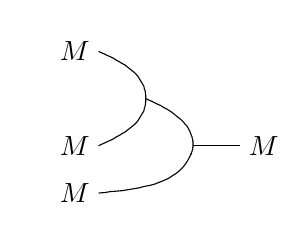
\begin{tikzpicture}[scale=0.60]
\useasboundingbox (-0.5,-0.5) rectangle (4.5,3.5);
\draw (2.00,2.00) -- (2.06,1.97) -- (2.13,1.94) -- (2.19,1.91) -- (2.25,1.88) -- (2.32,1.85) -- (2.38,1.81) -- (2.44,1.78) -- (2.49,1.75) -- (2.55,1.71) -- (2.60,1.67) -- (2.65,1.63) -- (2.70,1.59) -- (2.75,1.55) -- (2.79,1.51) -- (2.83,1.46) -- (2.87,1.42) -- (2.90,1.37) -- (2.93,1.31) -- (2.95,1.26) -- (2.97,1.20);
\draw (2.97,1.20) -- (2.98,1.19) -- (2.98,1.18) -- (2.98,1.17) -- (2.98,1.16) -- (2.99,1.15) -- (2.99,1.14) -- (2.99,1.13) -- (2.99,1.12) -- (2.99,1.11) -- (3.00,1.10) -- (3.00,1.09) -- (3.00,1.08) -- (3.00,1.07) -- (3.00,1.06) -- (3.00,1.05) -- (3.00,1.04) -- (3.00,1.03) -- (3.00,1.02) -- (3.00,1.01) -- (3.00,1.00);
\draw (3.00,1.00) -- (3.00,0.99) -- (3.00,0.98) -- (3.00,0.97) -- (3.00,0.96) -- (2.99,0.95) -- (2.99,0.94) -- (2.99,0.93) -- (2.99,0.92) -- (2.99,0.91) -- (2.98,0.90) -- (2.98,0.89) -- (2.98,0.88) -- (2.97,0.87) -- (2.97,0.86) -- (2.97,0.85) -- (2.96,0.84) -- (2.96,0.83) -- (2.96,0.82) -- (2.95,0.82) -- (2.95,0.81);
\draw (2.95,0.81) -- (2.90,0.71) -- (2.85,0.63) -- (2.79,0.55) -- (2.72,0.48) -- (2.65,0.42) -- (2.57,0.37) -- (2.48,0.31) -- (2.39,0.27) -- (2.29,0.23) -- (2.19,0.19) -- (2.08,0.16) -- (1.97,0.14) -- (1.86,0.11) -- (1.74,0.09) -- (1.62,0.07) -- (1.50,0.05) -- (1.38,0.04) -- (1.25,0.03) -- (1.13,0.01) -- (1.00,0.00);
\draw (1.00,3.00) -- (1.06,2.97) -- (1.13,2.94) -- (1.19,2.91) -- (1.26,2.88) -- (1.32,2.85) -- (1.38,2.81) -- (1.44,2.78) -- (1.50,2.74) -- (1.56,2.71) -- (1.61,2.67) -- (1.66,2.63) -- (1.71,2.59) -- (1.76,2.55) -- (1.80,2.51) -- (1.84,2.46) -- (1.87,2.41) -- (1.90,2.36) -- (1.93,2.31) -- (1.96,2.26) -- (1.97,2.20);
\draw (1.97,2.20) -- (1.98,2.19) -- (1.98,2.18) -- (1.98,2.17) -- (1.98,2.16) -- (1.99,2.15) -- (1.99,2.14) -- (1.99,2.13) -- (1.99,2.12) -- (1.99,2.11) -- (1.99,2.10) -- (1.99,2.09) -- (2.00,2.08) -- (2.00,2.07) -- (2.00,2.06) -- (2.00,2.05) -- (2.00,2.04) -- (2.00,2.03) -- (2.00,2.02) -- (2.00,2.01) -- (2.00,2.00);
\draw (2.00,2.00) -- (2.00,1.99) -- (2.00,1.98) -- (2.00,1.97) -- (2.00,1.96) -- (2.00,1.95) -- (2.00,1.94) -- (2.00,1.93) -- (2.00,1.92) -- (1.99,1.91) -- (1.99,1.90) -- (1.99,1.89) -- (1.99,1.88) -- (1.99,1.87) -- (1.99,1.86) -- (1.99,1.85) -- (1.98,1.84) -- (1.98,1.83) -- (1.98,1.82) -- (1.98,1.81) -- (1.97,1.80);
\draw (1.97,1.80) -- (1.96,1.74) -- (1.93,1.69) -- (1.90,1.64) -- (1.87,1.59) -- (1.84,1.54) -- (1.80,1.49) -- (1.76,1.45) -- (1.71,1.41) -- (1.66,1.37) -- (1.61,1.33) -- (1.56,1.29) -- (1.50,1.26) -- (1.44,1.22) -- (1.38,1.19) -- (1.32,1.15) -- (1.26,1.12) -- (1.19,1.09) -- (1.13,1.06) -- (1.06,1.03) -- (1.00,1.00);
\draw (3.00,1.00) -- (4.00,1.00);
\draw (0.50,3.00) node{$M$};
\draw (0.50,1.00) node{$M$};
\draw (4.50,1.00) node{$M$};
\draw (0.50,0.00) node{$M$};
\end{tikzpicture}
}}
\]
\end{verbatim}

\subsection{Visualizing your diagram}
Making a nice diagram is sometimes hard and \LaTeX{} compilation of the diagrams
usually takes some time to complete. If you want to quickly see the diagram
generated by \strid{} on a file \texttt{toto.strid}, type the command
\begin{center}
  \texttt{strid -g toto.strid}
\end{center}
This will open a window in which the output diagram is displayed, which is
refreshed every time the file \texttt{toto.strid} is changed.


\section{The operators}
\subsection{Line: \texttt{line}}
\[
\begin{tikzpicture}[scale=0.60]
\useasboundingbox (-0.5,-0.5) rectangle (0.5,4.5);
\draw (0.00,3.00) -- (0.00,2.95) -- (0.00,2.90) -- (0.00,2.85) -- (0.00,2.80) -- (0.00,2.75) -- (0.00,2.70) -- (0.00,2.65) -- (0.00,2.60) -- (0.00,2.55) -- (0.00,2.50) -- (0.00,2.45) -- (0.00,2.40) -- (0.00,2.35) -- (0.00,2.30) -- (0.00,2.25) -- (0.00,2.20) -- (0.00,2.15) -- (0.00,2.10) -- (0.00,2.05) -- (0.00,2.00);
\draw (0.00,2.00) -- (0.00,1.95) -- (0.00,1.90) -- (0.00,1.85) -- (0.00,1.80) -- (0.00,1.75) -- (0.00,1.70) -- (0.00,1.65) -- (0.00,1.60) -- (0.00,1.55) -- (0.00,1.50) -- (0.00,1.45) -- (0.00,1.40) -- (0.00,1.35) -- (0.00,1.30) -- (0.00,1.25) -- (0.00,1.20) -- (0.00,1.15) -- (0.00,1.10) -- (0.00,1.05) -- (0.00,1.00);
\draw (0.00,3.50) node{1};
\draw (0.00,0.50) node{2};
\end{tikzpicture}

\]
\subsection{Multiplication: \texttt{mult}}
\[
\begin{tikzpicture}[scale=0.60]
\useasboundingbox (-0.5,-0.5) rectangle (2.5,4.5);
\draw (1.00,2.00) -- (1.00,1.00);
\draw (0.00,3.00) -- (0.03,2.94) -- (0.06,2.87) -- (0.09,2.81) -- (0.12,2.74) -- (0.15,2.68) -- (0.19,2.62) -- (0.22,2.56) -- (0.26,2.50) -- (0.29,2.44) -- (0.33,2.39) -- (0.37,2.34) -- (0.41,2.29) -- (0.45,2.24) -- (0.49,2.20) -- (0.54,2.16) -- (0.59,2.13) -- (0.64,2.10) -- (0.69,2.07) -- (0.74,2.04) -- (0.80,2.03);
\draw (0.80,2.03) -- (0.81,2.02) -- (0.82,2.02) -- (0.83,2.02) -- (0.84,2.02) -- (0.85,2.01) -- (0.86,2.01) -- (0.87,2.01) -- (0.88,2.01) -- (0.89,2.01) -- (0.90,2.01) -- (0.91,2.01) -- (0.92,2.00) -- (0.93,2.00) -- (0.94,2.00) -- (0.95,2.00) -- (0.96,2.00) -- (0.97,2.00) -- (0.98,2.00) -- (0.99,2.00) -- (1.00,2.00);
\draw (1.00,2.00) -- (1.01,2.00) -- (1.02,2.00) -- (1.03,2.00) -- (1.04,2.00) -- (1.05,2.00) -- (1.06,2.00) -- (1.07,2.00) -- (1.08,2.00) -- (1.09,2.01) -- (1.10,2.01) -- (1.11,2.01) -- (1.12,2.01) -- (1.13,2.01) -- (1.14,2.01) -- (1.15,2.01) -- (1.16,2.02) -- (1.17,2.02) -- (1.18,2.02) -- (1.19,2.02) -- (1.20,2.03);
\draw (1.20,2.03) -- (1.26,2.04) -- (1.31,2.07) -- (1.36,2.10) -- (1.41,2.13) -- (1.46,2.16) -- (1.51,2.20) -- (1.55,2.24) -- (1.59,2.29) -- (1.63,2.34) -- (1.67,2.39) -- (1.71,2.44) -- (1.74,2.50) -- (1.78,2.56) -- (1.81,2.62) -- (1.85,2.68) -- (1.88,2.74) -- (1.91,2.81) -- (1.94,2.87) -- (1.97,2.94) -- (2.00,3.00);
\draw (0.00,3.50) node{$1$};
\draw (2.00,3.50) node{$2$};
\draw (1.00,0.50) node{$3$};
\end{tikzpicture}

\]
\subsection{Unit: \texttt{unit}}
\[
\begin{tikzpicture}[scale=0.60]
\useasboundingbox (-0.5,-0.5) rectangle (0.5,3.5);
\draw (0.00,2.00) -- (0.00,1.00);
\filldraw[fill=white] (0.00,2.00) ellipse (0.14cm and 0.14cm);
\draw (0.00,0.50) node{$1$};
\end{tikzpicture}

\]
\subsection{Adjunction: \texttt{adj}}
\[
\begin{tikzpicture}[scale=0.60]
\useasboundingbox (-0.5,-0.5) rectangle (2.5,2.5);
\draw (0.00,1.00) -- (0.05,1.07) -- (0.10,1.15) -- (0.15,1.22) -- (0.20,1.30) -- (0.25,1.37) -- (0.30,1.44) -- (0.35,1.50) -- (0.40,1.57) -- (0.45,1.63) -- (0.50,1.69) -- (0.55,1.74) -- (0.60,1.79) -- (0.65,1.84) -- (0.70,1.88) -- (0.75,1.91) -- (0.80,1.94) -- (0.85,1.97) -- (0.90,1.99) -- (0.95,2.00) -- (1.00,2.00);
\draw (1.00,2.00) -- (1.05,2.00) -- (1.10,1.99) -- (1.15,1.97) -- (1.20,1.94) -- (1.25,1.91) -- (1.30,1.88) -- (1.35,1.84) -- (1.40,1.79) -- (1.45,1.74) -- (1.50,1.69) -- (1.55,1.63) -- (1.60,1.57) -- (1.65,1.50) -- (1.70,1.44) -- (1.75,1.37) -- (1.80,1.30) -- (1.85,1.22) -- (1.90,1.15) -- (1.95,1.07) -- (2.00,1.00);
\draw (0.00,0.50) node{1};
\draw (2.00,0.50) node{2};
\end{tikzpicture}

\]
\subsection{Symmetry: \texttt{sym}}
\[
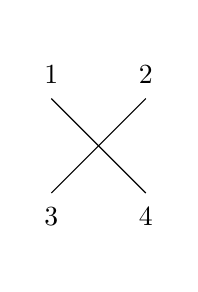
\begin{tikzpicture}[scale=0.60]
\useasboundingbox (-0.5,-0.5) rectangle (2.5,4.5);
\draw (0.00,3.00) -- (0.05,2.95) -- (0.10,2.90) -- (0.15,2.85) -- (0.20,2.80) -- (0.25,2.75) -- (0.30,2.70) -- (0.35,2.65) -- (0.40,2.60) -- (0.45,2.55) -- (0.50,2.50) -- (0.55,2.45) -- (0.60,2.40) -- (0.65,2.35) -- (0.70,2.30) -- (0.75,2.25) -- (0.80,2.20) -- (0.85,2.15) -- (0.90,2.10) -- (0.95,2.05) -- (1.00,2.00);
\draw (1.00,2.00) -- (1.05,1.95) -- (1.10,1.90) -- (1.15,1.85) -- (1.20,1.80) -- (1.25,1.75) -- (1.30,1.70) -- (1.35,1.65) -- (1.40,1.60) -- (1.45,1.55) -- (1.50,1.50) -- (1.55,1.45) -- (1.60,1.40) -- (1.65,1.35) -- (1.70,1.30) -- (1.75,1.25) -- (1.80,1.20) -- (1.85,1.15) -- (1.90,1.10) -- (1.95,1.05) -- (2.00,1.00);
\draw (2.00,3.00) -- (1.95,2.95) -- (1.90,2.90) -- (1.85,2.85) -- (1.80,2.80) -- (1.75,2.75) -- (1.70,2.70) -- (1.65,2.65) -- (1.60,2.60) -- (1.55,2.55) -- (1.50,2.50) -- (1.45,2.45) -- (1.40,2.40) -- (1.35,2.35) -- (1.30,2.30) -- (1.25,2.25) -- (1.20,2.20) -- (1.15,2.15) -- (1.10,2.10) -- (1.05,2.05) -- (1.00,2.00);
\draw (1.00,2.00) -- (0.95,1.95) -- (0.90,1.90) -- (0.85,1.85) -- (0.80,1.80) -- (0.75,1.75) -- (0.70,1.70) -- (0.65,1.65) -- (0.60,1.60) -- (0.55,1.55) -- (0.50,1.50) -- (0.45,1.45) -- (0.40,1.40) -- (0.35,1.35) -- (0.30,1.30) -- (0.25,1.25) -- (0.20,1.20) -- (0.15,1.15) -- (0.10,1.10) -- (0.05,1.05) -- (0.00,1.00);
\draw (0.00,3.50) node{1};
\draw (2.00,3.50) node{2};
\draw (0.00,0.50) node{3};
\draw (2.00,0.50) node{4};
\end{tikzpicture}

\]
\subsection{Braiding: \texttt{braid}}
\[
\begin{tikzpicture}[scale=0.60]
\useasboundingbox (-0.5,-0.5) rectangle (2.5,4.5);
\draw (2.00,3.00) -- (1.96,2.96) -- (1.91,2.91) -- (1.87,2.87) -- (1.83,2.83) -- (1.79,2.79) -- (1.74,2.74) -- (1.70,2.70) -- (1.66,2.66) -- (1.61,2.61) -- (1.57,2.57) -- (1.53,2.53) -- (1.48,2.48) -- (1.44,2.44) -- (1.40,2.40) -- (1.36,2.36) -- (1.31,2.31) -- (1.27,2.27) -- (1.23,2.23) -- (1.18,2.18) -- (1.14,2.14);
\draw (0.86,1.86) -- (0.82,1.82) -- (0.77,1.77) -- (0.73,1.73) -- (0.69,1.69) -- (0.64,1.64) -- (0.60,1.60) -- (0.56,1.56) -- (0.52,1.52) -- (0.47,1.47) -- (0.43,1.43) -- (0.39,1.39) -- (0.34,1.34) -- (0.30,1.30) -- (0.26,1.26) -- (0.21,1.21) -- (0.17,1.17) -- (0.13,1.13) -- (0.09,1.09) -- (0.04,1.04) -- (0.00,1.00);
\draw (0.00,3.00) -- (0.04,2.96) -- (0.09,2.91) -- (0.13,2.87) -- (0.17,2.83) -- (0.21,2.79) -- (0.26,2.74) -- (0.30,2.70) -- (0.34,2.66) -- (0.39,2.61) -- (0.43,2.57) -- (0.47,2.53) -- (0.52,2.48) -- (0.56,2.44) -- (0.60,2.40) -- (0.64,2.36) -- (0.69,2.31) -- (0.73,2.27) -- (0.77,2.23) -- (0.82,2.18) -- (0.86,2.14);
\draw (0.86,2.14) -- (0.87,2.13) -- (0.89,2.11) -- (0.90,2.10) -- (0.92,2.08) -- (0.93,2.07) -- (0.94,2.06) -- (0.96,2.04) -- (0.97,2.03) -- (0.99,2.01) -- (1.00,2.00) -- (1.01,1.99) -- (1.03,1.97) -- (1.04,1.96) -- (1.06,1.94) -- (1.07,1.93) -- (1.08,1.92) -- (1.10,1.90) -- (1.11,1.89) -- (1.13,1.87) -- (1.14,1.86);
\draw (1.14,1.86) -- (1.18,1.82) -- (1.23,1.77) -- (1.27,1.73) -- (1.31,1.69) -- (1.36,1.64) -- (1.40,1.60) -- (1.44,1.56) -- (1.48,1.52) -- (1.53,1.47) -- (1.57,1.43) -- (1.61,1.39) -- (1.66,1.34) -- (1.70,1.30) -- (1.74,1.26) -- (1.79,1.21) -- (1.83,1.17) -- (1.87,1.13) -- (1.91,1.09) -- (1.96,1.04) -- (2.00,1.00);
\draw (0.00,3.50) node{1};
\draw (2.00,3.50) node{2};
\draw (0.00,0.50) node{3};
\draw (2.00,0.50) node{4};
\end{tikzpicture}

\]
\subsection{$m,n$-ary box: \texttt{$m$box$n$}}
\[
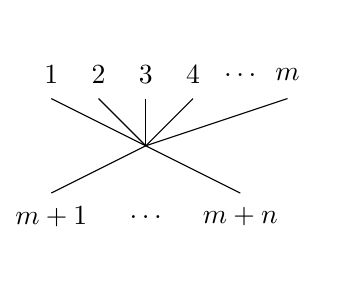
\begin{tikzpicture}[scale=0.60]
\useasboundingbox (-0.5,-0.5) rectangle (5.5,4.5);
\draw (2.00,2.00) -- (4.00,1.00);
\draw (2.00,2.00) -- (0.00,1.00);
\draw (5.00,3.00) -- (2.00,2.00);
\draw (3.00,3.00) -- (2.00,2.00);
\draw (2.00,3.00) -- (2.00,2.00);
\draw (1.00,3.00) -- (2.00,2.00);
\draw (0.00,3.00) -- (2.00,2.00);
\draw (0.00,3.50) node{$1$};
\draw (1.00,3.50) node{$2$};
\draw (2.00,3.50) node{$3$};
\draw (3.00,3.50) node{$4$};
\draw (4.00,3.50) node{$\ldots$};
\draw (5.00,3.50) node{$m$};
\draw (0.00,0.50) node{$m+1$};
\draw (2.00,0.50) node{$\ldots$};
\draw (4.00,0.50) node{$m+n$};
\end{tikzpicture}

\]
\subsection{Vertical box: \texttt{vbox}}
\[
\begin{tikzpicture}[scale=0.60]
\useasboundingbox (-0.5,-0.5) rectangle (4.5,5.5);
\draw (1.00,4.00) -- (2.00,4.00);
\draw (1.00,3.00) -- (2.00,3.00);
\draw (1.00,1.00) -- (2.00,1.00);
\draw (3.00,4.00) -- (2.00,4.00);
\draw (3.00,3.00) -- (2.00,3.00);
\draw (3.00,1.00) -- (2.00,1.00);
\filldraw[,fill=white] (1.50,0.50) rectangle (2.50,4.50);
\draw (0.50,4.00) node{$1$};
\draw (4.00,4.00) node{$m+1$};
\draw (0.50,3.00) node{$2$};
\draw (4.00,3.00) node{$m+2$};
\draw (0.50,2.00) node{$\vdots$};
\draw (3.50,2.00) node{$\vdots$};
\draw (0.50,1.00) node{$m$};
\draw (3.50,1.00) node{$n$};
\end{tikzpicture}

\]

\subsection{Region: \texttt{region}}
Regions can be delimited:
\[
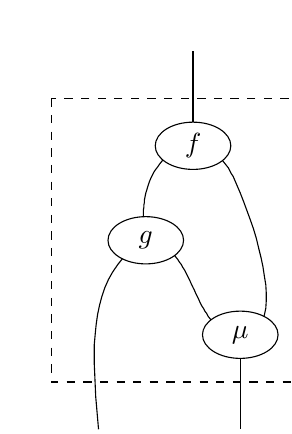
\begin{tikzpicture}[scale=0.60]
\useasboundingbox (-0.5,-0.5) rectangle (4.5,7.5);
\draw (3.00,5.00) -- (3.00,7.00);
\draw (2.00,3.00) -- (1.99,3.05) -- (1.99,3.10) -- (1.98,3.15) -- (1.98,3.20) -- (1.97,3.25) -- (1.97,3.30) -- (1.96,3.35) -- (1.96,3.40) -- (1.96,3.45) -- (1.95,3.50) -- (1.95,3.55) -- (1.95,3.60) -- (1.95,3.65) -- (1.96,3.70) -- (1.96,3.75) -- (1.97,3.80) -- (1.97,3.85) -- (1.98,3.90) -- (1.99,3.95) -- (2.00,4.00);
\draw (2.00,4.00) -- (2.02,4.06) -- (2.04,4.13) -- (2.06,4.19) -- (2.08,4.25) -- (2.11,4.32) -- (2.14,4.38) -- (2.17,4.44) -- (2.21,4.50) -- (2.25,4.55) -- (2.29,4.61) -- (2.33,4.66) -- (2.37,4.71) -- (2.42,4.75) -- (2.47,4.80) -- (2.52,4.84) -- (2.57,4.87) -- (2.63,4.90) -- (2.68,4.93) -- (2.74,4.96) -- (2.80,4.97);
\draw (2.80,4.97) -- (2.81,4.98) -- (2.82,4.98) -- (2.83,4.98) -- (2.84,4.98) -- (2.85,4.99) -- (2.86,4.99) -- (2.87,4.99) -- (2.88,4.99) -- (2.89,4.99) -- (2.90,4.99) -- (2.91,4.99) -- (2.92,5.00) -- (2.93,5.00) -- (2.94,5.00) -- (2.95,5.00) -- (2.96,5.00) -- (2.97,5.00) -- (2.98,5.00) -- (2.99,5.00) -- (3.00,5.00);
\draw (3.00,5.00) -- (3.01,5.00) -- (3.02,5.00) -- (3.03,5.00) -- (3.04,5.00) -- (3.05,5.00) -- (3.06,5.00) -- (3.07,5.00) -- (3.08,5.00) -- (3.09,4.99) -- (3.10,4.99) -- (3.11,4.99) -- (3.12,4.99) -- (3.13,4.99) -- (3.14,4.99) -- (3.15,4.99) -- (3.16,4.98) -- (3.17,4.98) -- (3.18,4.98) -- (3.19,4.98) -- (3.20,4.97);
\draw (3.20,4.97) -- (3.26,4.96) -- (3.31,4.94) -- (3.36,4.91) -- (3.41,4.88) -- (3.46,4.85) -- (3.51,4.81) -- (3.55,4.77) -- (3.59,4.73) -- (3.63,4.68) -- (3.67,4.63) -- (3.71,4.58) -- (3.75,4.53) -- (3.78,4.47) -- (3.81,4.41) -- (3.85,4.35) -- (3.88,4.28) -- (3.91,4.21) -- (3.94,4.14) -- (3.97,4.07) -- (4.00,4.00);
\draw (4.00,4.00) -- (4.07,3.82) -- (4.14,3.63) -- (4.21,3.44) -- (4.28,3.24) -- (4.34,3.04) -- (4.39,2.83) -- (4.44,2.63) -- (4.48,2.44) -- (4.51,2.24) -- (4.54,2.06) -- (4.55,1.88) -- (4.55,1.72) -- (4.54,1.56) -- (4.51,1.42) -- (4.47,1.30) -- (4.41,1.20) -- (4.34,1.11) -- (4.24,1.05) -- (4.13,1.01) -- (4.00,1.00);
\draw (4.00,1.00) -- (3.99,1.00) -- (3.98,1.00) -- (3.97,1.00) -- (3.96,1.00) -- (3.95,1.00) -- (3.94,1.00) -- (3.93,1.00) -- (3.92,1.00) -- (3.91,1.01) -- (3.90,1.01) -- (3.89,1.01) -- (3.88,1.01) -- (3.87,1.01) -- (3.86,1.01) -- (3.85,1.01) -- (3.84,1.02) -- (3.83,1.02) -- (3.82,1.02) -- (3.81,1.02) -- (3.80,1.03);
\draw (3.80,1.03) -- (3.74,1.04) -- (3.69,1.07) -- (3.63,1.10) -- (3.58,1.13) -- (3.53,1.16) -- (3.49,1.20) -- (3.44,1.25) -- (3.40,1.29) -- (3.36,1.34) -- (3.32,1.39) -- (3.29,1.45) -- (3.25,1.50) -- (3.22,1.56) -- (3.18,1.62) -- (3.15,1.68) -- (3.12,1.75) -- (3.09,1.81) -- (3.06,1.87) -- (3.03,1.94) -- (3.00,2.00);
\draw (3.00,2.00) -- (2.97,2.06) -- (2.94,2.13) -- (2.91,2.19) -- (2.88,2.25) -- (2.85,2.31) -- (2.82,2.37) -- (2.78,2.43) -- (2.75,2.49) -- (2.71,2.54) -- (2.68,2.59) -- (2.64,2.64) -- (2.60,2.69) -- (2.56,2.74) -- (2.51,2.78) -- (2.47,2.82) -- (2.42,2.86) -- (2.37,2.89) -- (2.31,2.92) -- (2.26,2.95) -- (2.20,2.97);
\draw (2.20,2.97) -- (2.19,2.98) -- (2.18,2.98) -- (2.17,2.98) -- (2.16,2.99) -- (2.15,2.99) -- (2.14,2.99) -- (2.13,2.99) -- (2.12,3.00) -- (2.11,3.00) -- (2.10,3.00) -- (2.09,3.00) -- (2.08,3.00) -- (2.07,3.00) -- (2.06,3.00) -- (2.05,3.00) -- (2.04,3.00) -- (2.03,3.00) -- (2.02,3.00) -- (2.01,3.00) -- (2.00,3.00);
\draw (2.00,3.00) -- (1.99,3.00) -- (1.98,3.00) -- (1.97,2.99) -- (1.96,2.99) -- (1.95,2.99) -- (1.94,2.98) -- (1.93,2.98) -- (1.93,2.97) -- (1.92,2.97) -- (1.91,2.96) -- (1.90,2.96) -- (1.89,2.95) -- (1.88,2.95) -- (1.87,2.94) -- (1.86,2.94) -- (1.86,2.93) -- (1.85,2.93) -- (1.84,2.92) -- (1.83,2.91) -- (1.82,2.91);
\draw (1.82,2.91) -- (1.67,2.78) -- (1.53,2.64) -- (1.41,2.49) -- (1.30,2.33) -- (1.21,2.17) -- (1.13,1.99) -- (1.07,1.81) -- (1.02,1.62) -- (0.98,1.43) -- (0.95,1.22) -- (0.93,1.02) -- (0.91,0.80) -- (0.91,0.59) -- (0.91,0.37) -- (0.92,0.15) -- (0.93,-0.08) -- (0.94,-0.31) -- (0.96,-0.54) -- (0.98,-0.77) -- (1.00,-1.00);
\draw (4.00,1.00) -- (4.00,-1.00);
\draw[dashed,] (0.00,6.00) rectangle (6.00,0.00);
\filldraw[fill=white] (3.00,5.00) ellipse (0.80cm and 0.50cm);
\filldraw[fill=white] (2.00,3.00) ellipse (0.80cm and 0.50cm);
\filldraw[fill=white] (4.00,1.00) ellipse (0.80cm and 0.50cm);
\draw (3.00,5.00) node{$f$};
\draw (2.00,3.00) node{$g$};
\draw (4.00,1.00) node{$\mu$};
\end{tikzpicture}

\]
is typeset by
\verbatiminput{pl_composition.strid}


\section{Parameters of operators}
\subsection{Labels}
Labels can be added to operators. For example the diagram
\[
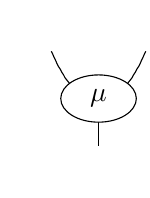
\begin{tikzpicture}[scale=0.60]
\useasboundingbox (-0.5,-0.5) rectangle (1.5,2.5);
\draw (1.00,1.00) -- (1.00,0.00);
\draw (0.00,2.00) -- (0.03,1.94) -- (0.06,1.87) -- (0.09,1.81) -- (0.12,1.74) -- (0.15,1.68) -- (0.19,1.62) -- (0.22,1.56) -- (0.26,1.50) -- (0.29,1.44) -- (0.33,1.39) -- (0.37,1.34) -- (0.41,1.29) -- (0.45,1.24) -- (0.49,1.20) -- (0.54,1.16) -- (0.59,1.13) -- (0.64,1.10) -- (0.69,1.07) -- (0.74,1.04) -- (0.80,1.03);
\draw (0.80,1.03) -- (0.81,1.02) -- (0.82,1.02) -- (0.83,1.02) -- (0.84,1.02) -- (0.85,1.01) -- (0.86,1.01) -- (0.87,1.01) -- (0.88,1.01) -- (0.89,1.01) -- (0.90,1.01) -- (0.91,1.01) -- (0.92,1.00) -- (0.93,1.00) -- (0.94,1.00) -- (0.95,1.00) -- (0.96,1.00) -- (0.97,1.00) -- (0.98,1.00) -- (0.99,1.00) -- (1.00,1.00);
\draw (1.00,1.00) -- (1.01,1.00) -- (1.02,1.00) -- (1.03,1.00) -- (1.04,1.00) -- (1.05,1.00) -- (1.06,1.00) -- (1.07,1.00) -- (1.08,1.00) -- (1.09,1.01) -- (1.10,1.01) -- (1.11,1.01) -- (1.12,1.01) -- (1.13,1.01) -- (1.14,1.01) -- (1.15,1.01) -- (1.16,1.02) -- (1.17,1.02) -- (1.18,1.02) -- (1.19,1.02) -- (1.20,1.03);
\draw (1.20,1.03) -- (1.26,1.04) -- (1.31,1.07) -- (1.36,1.10) -- (1.41,1.13) -- (1.46,1.16) -- (1.51,1.20) -- (1.55,1.24) -- (1.59,1.29) -- (1.63,1.34) -- (1.67,1.39) -- (1.71,1.44) -- (1.74,1.50) -- (1.78,1.56) -- (1.81,1.62) -- (1.85,1.68) -- (1.88,1.74) -- (1.91,1.81) -- (1.94,1.87) -- (1.97,1.94) -- (2.00,2.00);
\filldraw[fill=white] (1.00,1.00) ellipse (0.80cm and 0.50cm);
\draw (1.00,1.00) node{$\mu$};
\end{tikzpicture}

\]
can be typeset by \verbatiminput{mult_label.strid} If you don't like the size of
the ellipse surrounding the label, this can of course be changed. For example,
\[
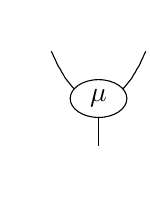
\begin{tikzpicture}[scale=0.60]
\useasboundingbox (-0.5,-0.5) rectangle (1.5,2.5);
\draw (1.00,1.00) -- (1.00,0.00);
\draw (0.00,2.00) -- (0.03,1.94) -- (0.06,1.87) -- (0.09,1.81) -- (0.12,1.74) -- (0.15,1.68) -- (0.19,1.62) -- (0.22,1.56) -- (0.26,1.50) -- (0.29,1.44) -- (0.33,1.39) -- (0.37,1.34) -- (0.41,1.29) -- (0.45,1.24) -- (0.49,1.20) -- (0.54,1.16) -- (0.59,1.13) -- (0.64,1.10) -- (0.69,1.07) -- (0.74,1.04) -- (0.80,1.03);
\draw (0.80,1.03) -- (0.81,1.02) -- (0.82,1.02) -- (0.83,1.02) -- (0.84,1.02) -- (0.85,1.01) -- (0.86,1.01) -- (0.87,1.01) -- (0.88,1.01) -- (0.89,1.01) -- (0.90,1.01) -- (0.91,1.01) -- (0.92,1.00) -- (0.93,1.00) -- (0.94,1.00) -- (0.95,1.00) -- (0.96,1.00) -- (0.97,1.00) -- (0.98,1.00) -- (0.99,1.00) -- (1.00,1.00);
\draw (1.00,1.00) -- (1.01,1.00) -- (1.02,1.00) -- (1.03,1.00) -- (1.04,1.00) -- (1.05,1.00) -- (1.06,1.00) -- (1.07,1.00) -- (1.08,1.00) -- (1.09,1.01) -- (1.10,1.01) -- (1.11,1.01) -- (1.12,1.01) -- (1.13,1.01) -- (1.14,1.01) -- (1.15,1.01) -- (1.16,1.02) -- (1.17,1.02) -- (1.18,1.02) -- (1.19,1.02) -- (1.20,1.03);
\draw (1.20,1.03) -- (1.26,1.04) -- (1.31,1.07) -- (1.36,1.10) -- (1.41,1.13) -- (1.46,1.16) -- (1.51,1.20) -- (1.55,1.24) -- (1.59,1.29) -- (1.63,1.34) -- (1.67,1.39) -- (1.71,1.44) -- (1.74,1.50) -- (1.78,1.56) -- (1.81,1.62) -- (1.85,1.68) -- (1.88,1.74) -- (1.91,1.81) -- (1.94,1.87) -- (1.97,1.94) -- (2.00,2.00);
\filldraw[fill=white] (1.00,1.00) ellipse (0.60cm and 0.40cm);
\draw (1.00,1.00) node{$\mu$};
\end{tikzpicture}

\]
can be typeset by
\verbatiminput{mult_small_label.strid}

Various shapes are available for labels:
\subsubsection{Triangles: \texttt{triangle} / \texttt{t}}
For example,
\[
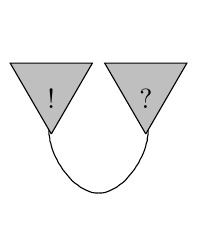
\begin{tikzpicture}[scale=0.60]
\useasboundingbox (-0.5,-0.5) rectangle (2.5,3.5);
\draw (0.00,2.00) -- (-0.01,1.95) -- (-0.01,1.90) -- (-0.02,1.85) -- (-0.03,1.80) -- (-0.03,1.75) -- (-0.04,1.70) -- (-0.04,1.65) -- (-0.05,1.60) -- (-0.05,1.56) -- (-0.05,1.51) -- (-0.06,1.46) -- (-0.06,1.41) -- (-0.05,1.36) -- (-0.05,1.31) -- (-0.05,1.25) -- (-0.04,1.20) -- (-0.03,1.15) -- (-0.03,1.10) -- (-0.01,1.05) -- (0.00,1.00);
\draw (0.00,1.00) -- (0.02,0.93) -- (0.05,0.85) -- (0.08,0.78) -- (0.12,0.71) -- (0.15,0.64) -- (0.20,0.57) -- (0.24,0.50) -- (0.29,0.44) -- (0.34,0.38) -- (0.39,0.32) -- (0.44,0.26) -- (0.50,0.21) -- (0.56,0.17) -- (0.62,0.12) -- (0.68,0.09) -- (0.74,0.06) -- (0.81,0.03) -- (0.87,0.01) -- (0.94,0.00) -- (1.00,0.00);
\draw (1.00,0.00) -- (1.06,0.00) -- (1.13,0.01) -- (1.19,0.03) -- (1.26,0.06) -- (1.32,0.09) -- (1.38,0.12) -- (1.44,0.17) -- (1.50,0.21) -- (1.56,0.26) -- (1.61,0.32) -- (1.66,0.38) -- (1.71,0.44) -- (1.76,0.50) -- (1.80,0.57) -- (1.85,0.64) -- (1.88,0.71) -- (1.92,0.78) -- (1.95,0.85) -- (1.98,0.93) -- (2.00,1.00);
\draw (2.00,1.00) -- (2.01,1.05) -- (2.03,1.10) -- (2.03,1.15) -- (2.04,1.20) -- (2.05,1.25) -- (2.05,1.31) -- (2.05,1.36) -- (2.06,1.41) -- (2.06,1.46) -- (2.05,1.51) -- (2.05,1.56) -- (2.05,1.60) -- (2.04,1.65) -- (2.04,1.70) -- (2.03,1.75) -- (2.03,1.80) -- (2.02,1.85) -- (2.01,1.90) -- (2.01,1.95) -- (2.00,2.00);
\filldraw[fill=lightgray] (0.00, 1.25)  -- (0.87,2.75) -- (-0.87,2.75) -- (0.00,1.25);
\filldraw[fill=lightgray] (2.00, 1.25)  -- (2.87,2.75) -- (1.13,2.75) -- (2.00,1.25);
\draw (0.00,2.00) node{$!$};
\draw (2.00,2.00) node{$?$};
\end{tikzpicture}

\]
can be typeset by
\verbatiminput{bang_maybe_cut.strid}

Here, the \texttt{s} parameter is the shape (currently, only \texttt{ellipse}
and \texttt{triangle} are available), the \texttt{d} parameter is the direction
of the triangle and the \texttt{c} parameter specifies the color of the
triangle.

\subsubsection{Rectangles: \texttt{rectangle} / \texttt{r}}
\[
\cinput{monoidal_bifunct_l.tex}
\quad=\quad
\cinput{monoidal_bifunct_r.tex}
\]
The left member is typeset by
\verbatiminput{monoidal_bifunct_l.strid}

\subsection{Arrows}
Lines can be oriented using the \texttt{a} attribute. For example,
\[
\begin{tikzpicture}[scale=0.60]
\useasboundingbox (-0.5,-0.5) rectangle (2.5,2.5);
\draw (1.00,1.00) -- (2.00,1.00);
\draw (1.40,1.10) -- (1.60,1.00);
\draw (1.40,0.90) -- (1.60,1.00);
\draw (0.00,2.00) -- (0.06,1.97) -- (0.13,1.94) -- (0.19,1.91) -- (0.26,1.88) -- (0.32,1.85) -- (0.38,1.81) -- (0.44,1.78) -- (0.50,1.74) -- (0.56,1.71) -- (0.61,1.67) -- (0.66,1.63) -- (0.71,1.59) -- (0.76,1.55) -- (0.80,1.51) -- (0.84,1.46) -- (0.87,1.41) -- (0.90,1.36) -- (0.93,1.31) -- (0.96,1.26) -- (0.97,1.20);
\draw (0.97,1.20) -- (0.98,1.19) -- (0.98,1.18) -- (0.98,1.17) -- (0.98,1.16) -- (0.99,1.15) -- (0.99,1.14) -- (0.99,1.13) -- (0.99,1.12) -- (0.99,1.11) -- (0.99,1.10) -- (0.99,1.09) -- (1.00,1.08) -- (1.00,1.07) -- (1.00,1.06) -- (1.00,1.05) -- (1.00,1.04) -- (1.00,1.03) -- (1.00,1.02) -- (1.00,1.01) -- (1.00,1.00);
\draw (1.00,1.00) -- (1.00,0.99) -- (1.00,0.98) -- (1.00,0.97) -- (1.00,0.96) -- (1.00,0.95) -- (1.00,0.94) -- (1.00,0.93) -- (1.00,0.92) -- (0.99,0.91) -- (0.99,0.90) -- (0.99,0.89) -- (0.99,0.88) -- (0.99,0.87) -- (0.99,0.86) -- (0.99,0.85) -- (0.98,0.84) -- (0.98,0.83) -- (0.98,0.82) -- (0.98,0.81) -- (0.97,0.80);
\draw (0.97,0.80) -- (0.96,0.74) -- (0.93,0.69) -- (0.90,0.64) -- (0.87,0.59) -- (0.84,0.54) -- (0.80,0.49) -- (0.76,0.45) -- (0.71,0.41) -- (0.66,0.37) -- (0.61,0.33) -- (0.56,0.29) -- (0.50,0.26) -- (0.44,0.22) -- (0.38,0.19) -- (0.32,0.15) -- (0.26,0.12) -- (0.19,0.09) -- (0.13,0.06) -- (0.06,0.03) -- (0.00,0.00);
\draw (0.64,0.23) -- (0.74,0.43);
\draw (0.52,0.39) -- (0.74,0.43);
\draw (0.59,1.81) -- (0.69,1.61);
\draw (0.47,1.65) -- (0.69,1.61);
\end{tikzpicture}

\]
can be typeset by \verbatiminput{mult_a.strid} To specify that the direction
should be backwards use the \texttt{d=b} subattribute. For example,
\[
\begin{tikzpicture}[scale=0.60]
\useasboundingbox (-0.5,-0.5) rectangle (2.5,2.5);
\draw (1.00,1.00) -- (2.00,1.00);
\draw (1.60,1.10) -- (1.40,1.00);
\draw (1.60,0.90) -- (1.40,1.00);
\draw (0.00,2.00) -- (0.06,1.97) -- (0.13,1.94) -- (0.19,1.91) -- (0.26,1.88) -- (0.32,1.85) -- (0.38,1.81) -- (0.44,1.78) -- (0.50,1.74) -- (0.56,1.71) -- (0.61,1.67) -- (0.66,1.63) -- (0.71,1.59) -- (0.76,1.55) -- (0.80,1.51) -- (0.84,1.46) -- (0.87,1.41) -- (0.90,1.36) -- (0.93,1.31) -- (0.96,1.26) -- (0.97,1.20);
\draw (0.97,1.20) -- (0.98,1.19) -- (0.98,1.18) -- (0.98,1.17) -- (0.98,1.16) -- (0.99,1.15) -- (0.99,1.14) -- (0.99,1.13) -- (0.99,1.12) -- (0.99,1.11) -- (0.99,1.10) -- (0.99,1.09) -- (1.00,1.08) -- (1.00,1.07) -- (1.00,1.06) -- (1.00,1.05) -- (1.00,1.04) -- (1.00,1.03) -- (1.00,1.02) -- (1.00,1.01) -- (1.00,1.00);
\draw (1.00,1.00) -- (1.00,0.99) -- (1.00,0.98) -- (1.00,0.97) -- (1.00,0.96) -- (1.00,0.95) -- (1.00,0.94) -- (1.00,0.93) -- (1.00,0.92) -- (0.99,0.91) -- (0.99,0.90) -- (0.99,0.89) -- (0.99,0.88) -- (0.99,0.87) -- (0.99,0.86) -- (0.99,0.85) -- (0.98,0.84) -- (0.98,0.83) -- (0.98,0.82) -- (0.98,0.81) -- (0.97,0.80);
\draw (0.97,0.80) -- (0.96,0.74) -- (0.93,0.69) -- (0.90,0.64) -- (0.87,0.59) -- (0.84,0.54) -- (0.80,0.49) -- (0.76,0.45) -- (0.71,0.41) -- (0.66,0.37) -- (0.61,0.33) -- (0.56,0.29) -- (0.50,0.26) -- (0.44,0.22) -- (0.38,0.19) -- (0.32,0.15) -- (0.26,0.12) -- (0.19,0.09) -- (0.13,0.06) -- (0.06,0.03) -- (0.00,0.00);
\draw (0.80,0.35) -- (0.58,0.31);
\draw (0.68,0.51) -- (0.58,0.31);
\draw (0.75,1.69) -- (0.53,1.73);
\draw (0.63,1.53) -- (0.53,1.73);
\end{tikzpicture}

\]
can by typeset by \verbatiminput{mult_ab.strid}


\section{Configuration files}
All parameters can be saved in a configuration file named
\texttt{strid.conf}. To generate a configuration file, type
\begin{verbatim}
strid --dump-conf
\end{verbatim}
You can then edit \texttt{strid.conf}.

Some of the options that can be set are:
\begin{itemize}
\item \verb+line_width+: default width of a line
\item \verb+label_width+: default width of a label
\item \verb+label_height+: default height of a label
\item \verb+no_tex_environment+: do not output \verb+\begin{tikz}+ and
    \verb+\end{tikz}+
\item \verb+scaling_factor+: scale the diagrams
\item \verb+label_triangle_height+: default height of a triangular label
\item \verb+label_rectangle_width+: default width of a rectangular label
\item \verb+label_rectangle_height+: default height of a rectangular label
\item \verb+interpolation+: interpolation method for drawing lines (possible
  values are \verb+cspline+ and \verb+linear+)
\item \verb+small_circle_ray+: ray of small circles (used to tweak the drawing
  of multiplications)
\end{itemize}

\section{Examples}
\subsection{Yang-Baxter equality for braids}
\[
\cinput{yang_baxter_l.tex}
\qquad=\qquad
\cinput{yang_baxter_r.tex}
\]
Left member is typeset by
\verbatiminput{yang_baxter_l.strid}
and right member by
\verbatiminput{yang_baxter_r.strid}

\subsection{Hopf law for bialgebras}
\[
\cinput{bialgebra_hopf_l.tex}
\quad=\quad
\cinput{bialgebra_hopf_r.tex}
\]
Left member is typeset by
\verbatiminput{bialgebra_hopf_l.strid}
and right member by
\verbatiminput{bialgebra_hopf_r.strid}

\newcommand{\A}{\mathbb{A}}
\newcommand{\B}{\mathbb{B}}
\newcommand{\C}{\mathbb{C}}
\subsection{Naturality condition for natural transformations between two lax functors between bicategories}

\begin{center}
\begin{tabular}{ccc}
{\scriptsize $\begin{tikzpicture}[scale=0.60]
\useasboundingbox (-0.5,-0.5) rectangle (8.5,17.5);
\draw (1.00,16.00) -- (1.00,15.95) -- (1.00,15.90) -- (1.00,15.85) -- (1.00,15.80) -- (0.99,15.75) -- (0.99,15.70) -- (0.99,15.65) -- (0.99,15.60) -- (0.99,15.55) -- (0.99,15.50) -- (0.99,15.45) -- (0.99,15.40) -- (0.99,15.35) -- (0.99,15.30) -- (0.99,15.25) -- (0.99,15.20) -- (0.99,15.15) -- (1.00,15.10) -- (1.00,15.05) -- (1.00,15.00);
\draw (1.00,15.00) -- (1.01,14.84) -- (1.02,14.68) -- (1.04,14.52) -- (1.06,14.36) -- (1.09,14.20) -- (1.12,14.04) -- (1.15,13.88) -- (1.19,13.72) -- (1.23,13.56) -- (1.27,13.41) -- (1.33,13.26) -- (1.38,13.10) -- (1.44,12.96) -- (1.51,12.81) -- (1.58,12.67) -- (1.65,12.53) -- (1.73,12.39) -- (1.81,12.25) -- (1.90,12.13) -- (2.00,12.00);
\draw (2.00,12.00) -- (2.04,11.95) -- (2.09,11.89) -- (2.14,11.84) -- (2.18,11.79) -- (2.23,11.73) -- (2.28,11.68) -- (2.33,11.63) -- (2.38,11.58) -- (2.43,11.53) -- (2.48,11.48) -- (2.53,11.43) -- (2.58,11.39) -- (2.63,11.34) -- (2.69,11.29) -- (2.74,11.24) -- (2.79,11.19) -- (2.84,11.14) -- (2.90,11.10) -- (2.95,11.05) -- (3.00,11.00);
\draw (3.00,11.00) -- (3.05,10.95) -- (3.10,10.90) -- (3.15,10.85) -- (3.21,10.80) -- (3.26,10.75) -- (3.31,10.71) -- (3.36,10.66) -- (3.41,10.61) -- (3.46,10.56) -- (3.51,10.51) -- (3.56,10.46) -- (3.61,10.40) -- (3.66,10.35) -- (3.70,10.30) -- (3.75,10.25) -- (3.80,10.20) -- (3.85,10.15) -- (3.90,10.10) -- (3.95,10.05) -- (4.00,10.00);
\draw (3.00,16.00) -- (3.00,15.95) -- (2.99,15.90) -- (2.99,15.85) -- (2.98,15.80) -- (2.98,15.74) -- (2.97,15.69) -- (2.97,15.64) -- (2.97,15.59) -- (2.97,15.54) -- (2.97,15.49) -- (2.96,15.44) -- (2.96,15.39) -- (2.97,15.34) -- (2.97,15.29) -- (2.97,15.24) -- (2.97,15.19) -- (2.98,15.14) -- (2.98,15.10) -- (2.99,15.05) -- (3.00,15.00);
\draw (3.00,15.00) -- (3.02,14.90) -- (3.05,14.81) -- (3.08,14.71) -- (3.12,14.62) -- (3.16,14.53) -- (3.20,14.44) -- (3.24,14.35) -- (3.29,14.26) -- (3.34,14.17) -- (3.40,14.08) -- (3.45,13.99) -- (3.50,13.90) -- (3.56,13.81) -- (3.61,13.72) -- (3.67,13.63) -- (3.72,13.54) -- (3.77,13.45) -- (3.82,13.36) -- (3.87,13.27) -- (3.91,13.18);
\draw (4.06,12.81) -- (4.09,12.75) -- (4.12,12.68) -- (4.15,12.62) -- (4.17,12.55) -- (4.20,12.49) -- (4.23,12.42) -- (4.26,12.36) -- (4.29,12.29) -- (4.31,12.22) -- (4.34,12.16) -- (4.37,12.09) -- (4.39,12.03) -- (4.41,11.96) -- (4.43,11.90) -- (4.45,11.83) -- (4.46,11.76) -- (4.48,11.70) -- (4.49,11.63) -- (4.50,11.57) -- (4.50,11.50);
\draw (4.50,11.50) -- (4.50,11.42) -- (4.50,11.35) -- (4.49,11.27) -- (4.48,11.20) -- (4.47,11.12) -- (4.45,11.05) -- (4.43,10.97) -- (4.41,10.90) -- (4.38,10.82) -- (4.36,10.75) -- (4.33,10.67) -- (4.30,10.60) -- (4.26,10.52) -- (4.23,10.45) -- (4.19,10.37) -- (4.15,10.30) -- (4.12,10.22) -- (4.08,10.15) -- (4.04,10.07) -- (4.00,10.00);
\draw (5.00,16.00) -- (4.99,15.95) -- (4.99,15.89) -- (4.98,15.84) -- (4.97,15.79) -- (4.97,15.74) -- (4.96,15.68) -- (4.96,15.63) -- (4.95,15.58) -- (4.95,15.53) -- (4.95,15.48) -- (4.94,15.43) -- (4.94,15.38) -- (4.95,15.33) -- (4.95,15.28) -- (4.95,15.23) -- (4.96,15.18) -- (4.97,15.14) -- (4.97,15.09) -- (4.99,15.04) -- (5.00,15.00);
\draw (5.00,15.00) -- (5.02,14.94) -- (5.05,14.88) -- (5.08,14.82) -- (5.12,14.77) -- (5.15,14.71) -- (5.20,14.66) -- (5.24,14.60) -- (5.29,14.55) -- (5.34,14.50) -- (5.39,14.45) -- (5.44,14.41) -- (5.50,14.36) -- (5.56,14.31) -- (5.62,14.27) -- (5.68,14.22) -- (5.74,14.18) -- (5.81,14.13) -- (5.87,14.09) -- (5.94,14.04) -- (6.00,14.00);
\draw (6.00,14.00) -- (6.06,14.04) -- (6.13,14.09) -- (6.19,14.13) -- (6.26,14.18) -- (6.32,14.22) -- (6.38,14.27) -- (6.44,14.31) -- (6.50,14.36) -- (6.56,14.41) -- (6.61,14.45) -- (6.66,14.50) -- (6.71,14.55) -- (6.76,14.60) -- (6.80,14.66) -- (6.85,14.71) -- (6.88,14.77) -- (6.92,14.82) -- (6.95,14.88) -- (6.98,14.94) -- (7.00,15.00);
\draw (7.00,15.00) -- (7.01,15.04) -- (7.03,15.09) -- (7.03,15.14) -- (7.04,15.18) -- (7.05,15.23) -- (7.05,15.28) -- (7.05,15.33) -- (7.06,15.38) -- (7.06,15.43) -- (7.05,15.48) -- (7.05,15.53) -- (7.05,15.58) -- (7.04,15.63) -- (7.04,15.68) -- (7.03,15.74) -- (7.03,15.79) -- (7.02,15.84) -- (7.01,15.89) -- (7.01,15.95) -- (7.00,16.00);
\draw (6.00,14.00) -- (6.04,13.95) -- (6.08,13.90) -- (6.12,13.85) -- (6.16,13.80) -- (6.19,13.75) -- (6.23,13.70) -- (6.27,13.65) -- (6.30,13.60) -- (6.33,13.55) -- (6.36,13.50) -- (6.39,13.45) -- (6.41,13.40) -- (6.44,13.35) -- (6.46,13.30) -- (6.47,13.25) -- (6.49,13.20) -- (6.49,13.15) -- (6.50,13.10) -- (6.50,13.05) -- (6.50,13.00);
\draw (6.50,13.00) -- (6.49,12.96) -- (6.49,12.92) -- (6.48,12.88) -- (6.46,12.83) -- (6.45,12.79) -- (6.43,12.75) -- (6.41,12.71) -- (6.39,12.67) -- (6.37,12.63) -- (6.35,12.59) -- (6.32,12.55) -- (6.30,12.50) -- (6.27,12.46) -- (6.24,12.42) -- (6.22,12.38) -- (6.19,12.34) -- (6.17,12.30) -- (6.14,12.26) -- (6.11,12.22) -- (6.09,12.18);
\draw (6.09,12.18) -- (6.08,12.16) -- (6.07,12.14) -- (6.06,12.13) -- (6.05,12.11) -- (6.04,12.09) -- (6.03,12.07) -- (6.02,12.06) -- (6.01,12.04) -- (6.00,12.02) -- (5.99,12.00) -- (5.98,11.99) -- (5.98,11.97) -- (5.97,11.95) -- (5.96,11.93) -- (5.95,11.91) -- (5.94,11.90) -- (5.93,11.88) -- (5.93,11.86) -- (5.92,11.84) -- (5.91,11.82);
\draw (5.91,11.82) -- (5.87,11.72) -- (5.84,11.62) -- (5.80,11.51) -- (5.77,11.41) -- (5.73,11.30) -- (5.70,11.19) -- (5.67,11.08) -- (5.63,10.97) -- (5.60,10.86) -- (5.56,10.76) -- (5.52,10.65) -- (5.48,10.56) -- (5.43,10.46) -- (5.38,10.37) -- (5.33,10.29) -- (5.28,10.22) -- (5.22,10.15) -- (5.15,10.09) -- (5.08,10.04) -- (5.00,10.00);
\draw (5.00,10.00) -- (4.96,9.98) -- (4.92,9.97) -- (4.87,9.96) -- (4.83,9.95) -- (4.78,9.94) -- (4.74,9.94) -- (4.69,9.94) -- (4.64,9.93) -- (4.59,9.93) -- (4.54,9.94) -- (4.49,9.94) -- (4.43,9.94) -- (4.38,9.95) -- (4.33,9.95) -- (4.27,9.96) -- (4.22,9.97) -- (4.17,9.97) -- (4.11,9.98) -- (4.06,9.99) -- (4.00,10.00);
\draw (6.00,14.00) -- (5.96,13.95) -- (5.92,13.90) -- (5.88,13.85) -- (5.84,13.80) -- (5.80,13.75) -- (5.77,13.70) -- (5.73,13.65) -- (5.70,13.60) -- (5.67,13.55) -- (5.64,13.50) -- (5.61,13.45) -- (5.58,13.40) -- (5.56,13.35) -- (5.54,13.30) -- (5.53,13.25) -- (5.51,13.20) -- (5.50,13.15) -- (5.50,13.10) -- (5.50,13.05) -- (5.50,13.00);
\draw (5.50,13.00) -- (5.51,12.96) -- (5.51,12.92) -- (5.53,12.88) -- (5.54,12.84) -- (5.55,12.79) -- (5.57,12.75) -- (5.59,12.71) -- (5.61,12.67) -- (5.64,12.63) -- (5.66,12.59) -- (5.68,12.55) -- (5.71,12.51) -- (5.73,12.47) -- (5.76,12.43) -- (5.79,12.38) -- (5.81,12.34) -- (5.84,12.30) -- (5.86,12.26) -- (5.89,12.22) -- (5.91,12.18);
\draw (6.09,11.82) -- (6.14,11.73) -- (6.19,11.64) -- (6.25,11.55) -- (6.30,11.46) -- (6.36,11.37) -- (6.42,11.28) -- (6.48,11.19) -- (6.54,11.10) -- (6.60,11.01) -- (6.65,10.91) -- (6.71,10.82) -- (6.76,10.73) -- (6.81,10.64) -- (6.85,10.55) -- (6.89,10.46) -- (6.93,10.37) -- (6.96,10.28) -- (6.98,10.18) -- (6.99,10.09) -- (7.00,10.00);
\draw (7.00,10.00) -- (7.00,9.91) -- (6.99,9.81) -- (6.97,9.72) -- (6.95,9.63) -- (6.92,9.54) -- (6.89,9.44) -- (6.85,9.35) -- (6.80,9.26) -- (6.76,9.16) -- (6.70,9.07) -- (6.65,8.98) -- (6.59,8.89) -- (6.53,8.80) -- (6.47,8.71) -- (6.40,8.62) -- (6.34,8.53) -- (6.28,8.44) -- (6.21,8.35) -- (6.15,8.26) -- (6.09,8.18);
\draw (5.86,7.86) -- (5.82,7.81) -- (5.78,7.77) -- (5.74,7.72) -- (5.70,7.67) -- (5.66,7.63) -- (5.62,7.59) -- (5.58,7.54) -- (5.54,7.50) -- (5.49,7.46) -- (5.45,7.42) -- (5.40,7.37) -- (5.36,7.33) -- (5.32,7.29) -- (5.27,7.25) -- (5.23,7.21) -- (5.18,7.17) -- (5.14,7.12) -- (5.09,7.08) -- (5.04,7.04) -- (5.00,7.00);
\draw (5.00,7.00) -- (4.95,6.95) -- (4.90,6.90) -- (4.85,6.85) -- (4.79,6.80) -- (4.74,6.76) -- (4.69,6.71) -- (4.64,6.66) -- (4.59,6.61) -- (4.54,6.56) -- (4.49,6.51) -- (4.44,6.46) -- (4.39,6.41) -- (4.34,6.35) -- (4.29,6.30) -- (4.25,6.25) -- (4.20,6.20) -- (4.15,6.15) -- (4.10,6.10) -- (4.05,6.05) -- (4.00,6.00);
\draw (6.00,14.00) -- (5.95,13.98) -- (5.90,13.95) -- (5.85,13.93) -- (5.80,13.90) -- (5.75,13.88) -- (5.70,13.85) -- (5.65,13.83) -- (5.60,13.80) -- (5.55,13.78) -- (5.50,13.75) -- (5.45,13.73) -- (5.40,13.70) -- (5.35,13.68) -- (5.30,13.65) -- (5.25,13.63) -- (5.20,13.60) -- (5.15,13.58) -- (5.10,13.55) -- (5.05,13.53) -- (5.00,13.50);
\draw (5.00,13.50) -- (4.96,13.48) -- (4.92,13.46) -- (4.88,13.44) -- (4.84,13.42) -- (4.79,13.40) -- (4.75,13.38) -- (4.71,13.36) -- (4.67,13.34) -- (4.63,13.31) -- (4.59,13.29) -- (4.55,13.27) -- (4.51,13.25) -- (4.47,13.23) -- (4.43,13.21) -- (4.38,13.19) -- (4.34,13.17) -- (4.30,13.15) -- (4.26,13.13) -- (4.22,13.11) -- (4.18,13.09);
\draw (4.18,13.09) -- (4.16,13.08) -- (4.14,13.07) -- (4.13,13.06) -- (4.11,13.05) -- (4.09,13.04) -- (4.07,13.04) -- (4.05,13.03) -- (4.04,13.02) -- (4.02,13.01) -- (4.00,13.00) -- (3.98,12.99) -- (3.96,12.98) -- (3.95,12.97) -- (3.93,12.96) -- (3.91,12.96) -- (3.89,12.95) -- (3.87,12.94) -- (3.86,12.93) -- (3.84,12.92) -- (3.82,12.91);
\draw (3.82,12.91) -- (3.78,12.89) -- (3.74,12.87) -- (3.70,12.85) -- (3.66,12.83) -- (3.62,12.81) -- (3.58,12.78) -- (3.54,12.76) -- (3.49,12.74) -- (3.45,12.72) -- (3.41,12.70) -- (3.37,12.68) -- (3.33,12.66) -- (3.29,12.64) -- (3.25,12.62) -- (3.21,12.60) -- (3.17,12.58) -- (3.12,12.56) -- (3.08,12.54) -- (3.04,12.52) -- (3.00,12.50);
\draw (3.00,12.50) -- (2.95,12.48) -- (2.90,12.45) -- (2.85,12.43) -- (2.79,12.41) -- (2.74,12.39) -- (2.69,12.37) -- (2.64,12.34) -- (2.59,12.32) -- (2.54,12.30) -- (2.49,12.27) -- (2.44,12.25) -- (2.39,12.23) -- (2.34,12.20) -- (2.29,12.18) -- (2.24,12.15) -- (2.19,12.12) -- (2.14,12.09) -- (2.09,12.06) -- (2.05,12.03) -- (2.00,12.00);
\draw (2.00,12.00) -- (1.91,11.93) -- (1.82,11.86) -- (1.74,11.78) -- (1.66,11.70) -- (1.58,11.61) -- (1.51,11.52) -- (1.44,11.42) -- (1.38,11.32) -- (1.32,11.22) -- (1.26,11.12) -- (1.21,11.01) -- (1.17,10.90) -- (1.12,10.79) -- (1.09,10.68) -- (1.06,10.57) -- (1.04,10.45) -- (1.02,10.34) -- (1.01,10.23) -- (1.00,10.11) -- (1.00,10.00);
\draw (1.00,10.00) -- (1.01,9.89) -- (1.02,9.78) -- (1.04,9.67) -- (1.06,9.56) -- (1.10,9.45) -- (1.13,9.35) -- (1.17,9.24) -- (1.22,9.14) -- (1.27,9.03) -- (1.32,8.93) -- (1.37,8.83) -- (1.43,8.73) -- (1.50,8.64) -- (1.56,8.54) -- (1.63,8.45) -- (1.70,8.35) -- (1.77,8.26) -- (1.85,8.17) -- (1.92,8.09) -- (2.00,8.00);
\draw (2.00,8.00) -- (2.05,7.95) -- (2.10,7.89) -- (2.15,7.84) -- (2.20,7.79) -- (2.25,7.74) -- (2.29,7.69) -- (2.34,7.64) -- (2.39,7.59) -- (2.44,7.54) -- (2.49,7.49) -- (2.55,7.44) -- (2.60,7.39) -- (2.65,7.34) -- (2.70,7.29) -- (2.75,7.24) -- (2.80,7.19) -- (2.85,7.15) -- (2.90,7.10) -- (2.95,7.05) -- (3.00,7.00);
\draw (3.00,7.00) -- (3.05,6.95) -- (3.10,6.90) -- (3.15,6.85) -- (3.20,6.80) -- (3.25,6.75) -- (3.30,6.70) -- (3.35,6.65) -- (3.40,6.60) -- (3.45,6.55) -- (3.50,6.50) -- (3.55,6.45) -- (3.60,6.40) -- (3.65,6.35) -- (3.70,6.30) -- (3.75,6.25) -- (3.80,6.20) -- (3.85,6.15) -- (3.90,6.10) -- (3.95,6.05) -- (4.00,6.00);
\draw (4.00,10.00) -- (4.05,9.95) -- (4.10,9.90) -- (4.15,9.85) -- (4.20,9.80) -- (4.25,9.75) -- (4.30,9.70) -- (4.35,9.65) -- (4.40,9.60) -- (4.45,9.55) -- (4.50,9.50) -- (4.55,9.45) -- (4.60,9.40) -- (4.65,9.35) -- (4.70,9.30) -- (4.75,9.25) -- (4.80,9.20) -- (4.85,9.15) -- (4.90,9.10) -- (4.95,9.05) -- (5.00,9.00);
\draw (5.00,9.00) -- (5.04,8.96) -- (5.09,8.91) -- (5.13,8.87) -- (5.17,8.83) -- (5.22,8.79) -- (5.26,8.74) -- (5.30,8.70) -- (5.34,8.66) -- (5.39,8.61) -- (5.43,8.57) -- (5.47,8.53) -- (5.52,8.49) -- (5.56,8.44) -- (5.60,8.40) -- (5.64,8.36) -- (5.69,8.31) -- (5.73,8.27) -- (5.77,8.23) -- (5.82,8.18) -- (5.86,8.14);
\draw (5.86,8.14) -- (5.87,8.13) -- (5.89,8.11) -- (5.90,8.10) -- (5.91,8.08) -- (5.93,8.07) -- (5.94,8.06) -- (5.96,8.04) -- (5.97,8.03) -- (5.99,8.01) -- (6.00,8.00) -- (6.01,7.99) -- (6.03,7.97) -- (6.04,7.96) -- (6.06,7.94) -- (6.07,7.93) -- (6.08,7.91) -- (6.10,7.90) -- (6.11,7.89) -- (6.13,7.87) -- (6.14,7.86);
\draw (6.14,7.86) -- (6.19,7.82) -- (6.23,7.77) -- (6.27,7.73) -- (6.32,7.69) -- (6.36,7.65) -- (6.41,7.61) -- (6.45,7.56) -- (6.50,7.52) -- (6.54,7.48) -- (6.59,7.44) -- (6.63,7.40) -- (6.67,7.35) -- (6.72,7.31) -- (6.76,7.27) -- (6.80,7.22) -- (6.84,7.18) -- (6.88,7.14) -- (6.92,7.09) -- (6.96,7.05) -- (7.00,7.00);
\draw (7.00,7.00) -- (7.12,6.84) -- (7.23,6.67) -- (7.34,6.50) -- (7.43,6.32) -- (7.51,6.13) -- (7.59,5.94) -- (7.65,5.75) -- (7.71,5.55) -- (7.76,5.34) -- (7.81,5.14) -- (7.85,4.93) -- (7.88,4.72) -- (7.91,4.50) -- (7.93,4.29) -- (7.95,4.07) -- (7.97,3.86) -- (7.98,3.64) -- (7.99,3.43) -- (7.99,3.21) -- (8.00,3.00);
\draw (8.00,3.00) -- (8.00,2.90) -- (8.00,2.80) -- (8.00,2.69) -- (8.01,2.59) -- (8.01,2.49) -- (8.01,2.39) -- (8.01,2.29) -- (8.01,2.19) -- (8.01,2.09) -- (8.01,1.99) -- (8.01,1.89) -- (8.01,1.79) -- (8.01,1.69) -- (8.01,1.59) -- (8.00,1.49) -- (8.00,1.39) -- (8.00,1.30) -- (8.00,1.20) -- (8.00,1.10) -- (8.00,1.00);
\draw (4.00,10.00) -- (4.00,9.90) -- (4.00,9.80) -- (4.00,9.70) -- (4.00,9.60) -- (4.00,9.50) -- (4.00,9.40) -- (4.00,9.30) -- (4.00,9.20) -- (4.00,9.10) -- (4.00,9.00) -- (4.00,8.90) -- (4.00,8.80) -- (4.00,8.70) -- (4.00,8.60) -- (4.00,8.50) -- (4.00,8.40) -- (4.00,8.30) -- (4.00,8.20) -- (4.00,8.10) -- (4.00,8.00);
\draw (4.00,8.00) -- (4.00,7.90) -- (4.00,7.80) -- (4.00,7.70) -- (4.00,7.60) -- (4.00,7.50) -- (4.00,7.40) -- (4.00,7.30) -- (4.00,7.20) -- (4.00,7.10) -- (4.00,7.00) -- (4.00,6.90) -- (4.00,6.80) -- (4.00,6.70) -- (4.00,6.60) -- (4.00,6.50) -- (4.00,6.40) -- (4.00,6.30) -- (4.00,6.20) -- (4.00,6.10) -- (4.00,6.00);
\draw (4.00,10.00) -- (3.95,9.95) -- (3.90,9.90) -- (3.85,9.85) -- (3.80,9.80) -- (3.75,9.75) -- (3.70,9.70) -- (3.65,9.65) -- (3.60,9.60) -- (3.55,9.55) -- (3.50,9.49) -- (3.45,9.44) -- (3.40,9.39) -- (3.35,9.34) -- (3.30,9.30) -- (3.25,9.25) -- (3.20,9.20) -- (3.15,9.15) -- (3.10,9.10) -- (3.05,9.05) -- (3.00,9.00);
\draw (3.00,9.00) -- (2.95,8.95) -- (2.90,8.90) -- (2.85,8.85) -- (2.80,8.81) -- (2.75,8.76) -- (2.70,8.71) -- (2.65,8.66) -- (2.59,8.61) -- (2.54,8.56) -- (2.49,8.52) -- (2.44,8.47) -- (2.39,8.42) -- (2.34,8.37) -- (2.29,8.32) -- (2.24,8.26) -- (2.19,8.21) -- (2.15,8.16) -- (2.10,8.11) -- (2.05,8.05) -- (2.00,8.00);
\draw (2.00,8.00) -- (1.92,7.91) -- (1.85,7.82) -- (1.78,7.73) -- (1.71,7.64) -- (1.64,7.54) -- (1.57,7.45) -- (1.50,7.35) -- (1.44,7.25) -- (1.38,7.15) -- (1.33,7.05) -- (1.27,6.95) -- (1.22,6.85) -- (1.18,6.74) -- (1.14,6.64) -- (1.10,6.53) -- (1.07,6.43) -- (1.05,6.32) -- (1.02,6.21) -- (1.01,6.11) -- (1.00,6.00);
\draw (1.00,6.00) -- (1.00,5.89) -- (1.00,5.79) -- (1.01,5.68) -- (1.02,5.57) -- (1.04,5.47) -- (1.07,5.36) -- (1.10,5.26) -- (1.14,5.15) -- (1.18,5.05) -- (1.23,4.95) -- (1.28,4.85) -- (1.34,4.75) -- (1.41,4.65) -- (1.48,4.55) -- (1.55,4.46) -- (1.63,4.36) -- (1.72,4.27) -- (1.81,4.18) -- (1.90,4.09) -- (2.00,4.00);
\draw (2.00,4.00) -- (2.06,3.95) -- (2.13,3.89) -- (2.20,3.84) -- (2.27,3.79) -- (2.33,3.74) -- (2.40,3.68) -- (2.47,3.63) -- (2.53,3.58) -- (2.59,3.53) -- (2.65,3.48) -- (2.71,3.44) -- (2.76,3.39) -- (2.81,3.34) -- (2.86,3.29) -- (2.90,3.24) -- (2.93,3.19) -- (2.96,3.15) -- (2.98,3.10) -- (2.99,3.05) -- (3.00,3.00);
\draw (3.00,3.00) -- (3.00,2.95) -- (2.99,2.90) -- (2.98,2.85) -- (2.95,2.80) -- (2.92,2.75) -- (2.89,2.70) -- (2.85,2.66) -- (2.80,2.61) -- (2.75,2.56) -- (2.70,2.51) -- (2.64,2.45) -- (2.58,2.40) -- (2.51,2.35) -- (2.44,2.30) -- (2.37,2.25) -- (2.30,2.20) -- (2.23,2.15) -- (2.15,2.10) -- (2.08,2.05) -- (2.00,2.00);
\draw (4.00,6.00) -- (4.13,5.97) -- (4.26,5.94) -- (4.38,5.90) -- (4.51,5.87) -- (4.63,5.83) -- (4.76,5.80) -- (4.88,5.76) -- (4.99,5.72) -- (5.11,5.68) -- (5.21,5.63) -- (5.32,5.59) -- (5.42,5.54) -- (5.52,5.48) -- (5.60,5.43) -- (5.69,5.37) -- (5.77,5.30) -- (5.84,5.23) -- (5.90,5.16) -- (5.95,5.08) -- (6.00,5.00);
\draw (6.00,5.00) -- (6.03,4.92) -- (6.06,4.84) -- (6.09,4.75) -- (6.10,4.66) -- (6.11,4.57) -- (6.12,4.48) -- (6.13,4.38) -- (6.12,4.28) -- (6.12,4.17) -- (6.11,4.07) -- (6.11,3.97) -- (6.10,3.86) -- (6.08,3.75) -- (6.07,3.64) -- (6.06,3.54) -- (6.04,3.43) -- (6.03,3.32) -- (6.02,3.21) -- (6.01,3.11) -- (6.00,3.00);
\draw (6.00,3.00) -- (6.00,2.95) -- (5.99,2.90) -- (5.99,2.84) -- (5.99,2.79) -- (5.99,2.74) -- (5.99,2.69) -- (5.99,2.64) -- (5.99,2.59) -- (5.99,2.54) -- (5.99,2.49) -- (5.99,2.44) -- (5.99,2.39) -- (5.99,2.34) -- (5.99,2.29) -- (5.99,2.24) -- (5.99,2.20) -- (5.99,2.15) -- (6.00,2.10) -- (6.00,2.05) -- (6.00,2.00);
\draw (4.00,6.00) -- (4.00,5.95) -- (4.00,5.90) -- (4.00,5.85) -- (4.00,5.80) -- (4.00,5.75) -- (4.00,5.70) -- (4.00,5.65) -- (4.00,5.60) -- (4.00,5.55) -- (4.00,5.50) -- (4.00,5.45) -- (4.00,5.40) -- (4.00,5.35) -- (4.00,5.30) -- (4.00,5.25) -- (4.00,5.20) -- (4.00,5.15) -- (4.00,5.10) -- (4.00,5.05) -- (4.00,5.00);
\draw (4.00,5.00) -- (4.00,4.90) -- (4.00,4.80) -- (4.00,4.70) -- (4.00,4.60) -- (4.00,4.50) -- (4.00,4.40) -- (4.00,4.30) -- (4.00,4.20) -- (4.00,4.10) -- (4.00,4.00) -- (4.00,3.90) -- (4.00,3.80) -- (4.00,3.70) -- (4.00,3.60) -- (4.00,3.50) -- (4.00,3.40) -- (4.00,3.30) -- (4.00,3.20) -- (4.00,3.10) -- (4.00,3.00);
\draw (4.00,3.00) -- (4.00,2.90) -- (4.00,2.80) -- (4.00,2.70) -- (4.00,2.60) -- (4.00,2.50) -- (4.00,2.40) -- (4.00,2.30) -- (4.00,2.20) -- (4.00,2.10) -- (4.00,2.00) -- (4.00,1.90) -- (4.00,1.80) -- (4.00,1.70) -- (4.00,1.60) -- (4.00,1.50) -- (4.00,1.40) -- (4.00,1.30) -- (4.00,1.20) -- (4.00,1.10) -- (4.00,1.00);
\draw (4.00,6.00) -- (3.95,5.95) -- (3.90,5.90) -- (3.85,5.85) -- (3.79,5.81) -- (3.74,5.76) -- (3.69,5.71) -- (3.64,5.66) -- (3.59,5.61) -- (3.54,5.56) -- (3.49,5.51) -- (3.44,5.46) -- (3.39,5.41) -- (3.34,5.36) -- (3.29,5.31) -- (3.24,5.26) -- (3.19,5.21) -- (3.14,5.16) -- (3.09,5.11) -- (3.05,5.05) -- (3.00,5.00);
\draw (3.00,5.00) -- (2.95,4.95) -- (2.91,4.89) -- (2.86,4.84) -- (2.82,4.78) -- (2.77,4.73) -- (2.72,4.68) -- (2.68,4.62) -- (2.63,4.57) -- (2.59,4.52) -- (2.54,4.46) -- (2.49,4.41) -- (2.44,4.36) -- (2.39,4.31) -- (2.34,4.26) -- (2.29,4.22) -- (2.23,4.17) -- (2.18,4.12) -- (2.12,4.08) -- (2.06,4.04) -- (2.00,4.00);
\draw (2.00,4.00) -- (1.90,3.94) -- (1.80,3.89) -- (1.69,3.83) -- (1.58,3.79) -- (1.46,3.74) -- (1.35,3.70) -- (1.24,3.66) -- (1.12,3.62) -- (1.01,3.57) -- (0.89,3.53) -- (0.78,3.49) -- (0.68,3.45) -- (0.57,3.41) -- (0.47,3.36) -- (0.38,3.31) -- (0.29,3.26) -- (0.20,3.20) -- (0.13,3.14) -- (0.06,3.07) -- (0.00,3.00);
\draw (0.00,3.00) -- (-0.05,2.93) -- (-0.08,2.86) -- (-0.12,2.78) -- (-0.14,2.69) -- (-0.16,2.61) -- (-0.18,2.52) -- (-0.18,2.42) -- (-0.19,2.33) -- (-0.19,2.23) -- (-0.18,2.12) -- (-0.18,2.02) -- (-0.17,1.91) -- (-0.15,1.80) -- (-0.13,1.69) -- (-0.12,1.58) -- (-0.09,1.46) -- (-0.07,1.35) -- (-0.05,1.23) -- (-0.02,1.12) -- (0.00,1.00);
\filldraw[fill=white] (6.00,14.00) ellipse (0.80cm and 0.50cm);
\filldraw[fill=white] (2.00,12.00) ellipse (0.80cm and 0.50cm);
\filldraw[fill=white] (4.00,10.00) ellipse (1.60cm and 0.80cm);
\filldraw[fill=white] (2.00,8.00) ellipse (0.80cm and 0.50cm);
\filldraw[fill=white] (4.00,6.00) ellipse (1.60cm and 0.80cm);
\filldraw[fill=white] (2.00,4.00) ellipse (0.80cm and 0.50cm);
\draw (1.00,16.50) node{$\circ$};
\draw (3.00,16.50) node{$[\![\mathcal{G}\A,\mathcal{G}\C]\!] \times \theta_\A$};
\draw (5.00,16.50) node{$\mathcal{G}$};
\draw (7.00,16.50) node{$\circ$};
\draw (6.00,14.00) node{$\tilde{\mathcal{G}}_2$};
\draw (2.00,12.00) node{$\alpha$};
\draw (4.00,10.00) node{$[\![\mathcal{G}\B,\mathcal{G}\C]\!] \times \theta$};
\draw (2.00,8.00) node{$\alpha^{-1}$};
\draw (4.00,6.00) node{$\theta \times [\![\mathcal{F}\A,\mathcal{F}\B]\!]$};
\draw (2.00,4.00) node{$\alpha$};
\draw (2.00,1.50) node{$[\![\mathcal{F}\C,\mathcal{G}\C]\!] \times \circ$};
\draw (6.00,1.50) node{$\mathcal{F} \times [\![\mathcal{F}\A,\mathcal{F}\B]\!]$};
\draw (0.00,0.50) node{$\circ$};
\draw (4.00,0.50) node{$\theta_\C \times [\![\mathcal{F}\B,\mathcal{F}\C]\!]
\times [\![\mathcal{F}\A,\mathcal{F}\B]\!]$};
\draw (8.00,0.50) node{$\qquad [\![B,C]\!] \times \mathcal{F}$};
\end{tikzpicture}
$}
&
\qquad
\raisebox{5cm}{$=$}
\qquad
&
{\scriptsize $\begin{tikzpicture}[scale=0.60]
\useasboundingbox (-0.5,-0.5) rectangle (8.5,17.5);
\draw (1.00,16.00) -- (1.00,15.95) -- (1.00,15.90) -- (1.00,15.85) -- (1.00,15.80) -- (1.01,15.75) -- (1.01,15.70) -- (1.01,15.65) -- (1.01,15.60) -- (1.01,15.55) -- (1.01,15.50) -- (1.01,15.45) -- (1.01,15.40) -- (1.01,15.35) -- (1.01,15.30) -- (1.01,15.25) -- (1.01,15.20) -- (1.01,15.15) -- (1.00,15.10) -- (1.00,15.05) -- (1.00,15.00);
\draw (1.00,15.00) -- (1.00,14.95) -- (0.99,14.90) -- (0.99,14.85) -- (0.99,14.80) -- (0.99,14.74) -- (0.98,14.69) -- (0.98,14.64) -- (0.98,14.59) -- (0.97,14.54) -- (0.97,14.49) -- (0.97,14.44) -- (0.97,14.39) -- (0.97,14.34) -- (0.97,14.29) -- (0.97,14.24) -- (0.98,14.19) -- (0.98,14.14) -- (0.99,14.09) -- (0.99,14.05) -- (1.00,14.00);
\draw (1.00,14.00) -- (1.03,13.87) -- (1.07,13.75) -- (1.12,13.63) -- (1.18,13.51) -- (1.25,13.40) -- (1.33,13.29) -- (1.41,13.18) -- (1.51,13.08) -- (1.61,12.98) -- (1.71,12.88) -- (1.83,12.79) -- (1.94,12.69) -- (2.07,12.60) -- (2.19,12.51) -- (2.32,12.43) -- (2.45,12.34) -- (2.59,12.25) -- (2.72,12.17) -- (2.86,12.08) -- (3.00,12.00);
\draw (3.00,16.00) -- (3.00,15.95) -- (3.00,15.90) -- (3.00,15.85) -- (3.00,15.80) -- (3.00,15.75) -- (3.00,15.70) -- (3.00,15.65) -- (3.00,15.60) -- (3.00,15.55) -- (3.00,15.50) -- (3.00,15.45) -- (3.00,15.40) -- (3.00,15.35) -- (3.00,15.30) -- (3.00,15.25) -- (3.00,15.20) -- (3.00,15.15) -- (3.00,15.10) -- (3.00,15.05) -- (3.00,15.00);
\draw (3.00,15.00) -- (3.00,14.95) -- (3.00,14.90) -- (3.00,14.85) -- (3.00,14.80) -- (3.00,14.75) -- (3.00,14.70) -- (3.00,14.65) -- (3.00,14.60) -- (3.00,14.55) -- (3.00,14.50) -- (3.00,14.45) -- (3.00,14.40) -- (3.00,14.35) -- (3.00,14.30) -- (3.00,14.25) -- (3.00,14.20) -- (3.00,14.15) -- (3.00,14.10) -- (3.00,14.05) -- (3.00,14.00);
\draw (3.00,14.00) -- (3.00,13.90) -- (3.00,13.80) -- (3.00,13.70) -- (3.00,13.60) -- (3.00,13.50) -- (3.00,13.40) -- (3.00,13.30) -- (3.00,13.20) -- (3.00,13.10) -- (3.00,13.00) -- (3.00,12.90) -- (3.00,12.80) -- (3.00,12.70) -- (3.00,12.60) -- (3.00,12.50) -- (3.00,12.40) -- (3.00,12.30) -- (3.00,12.20) -- (3.00,12.10) -- (3.00,12.00);
\draw (5.00,16.00) -- (5.00,15.95) -- (5.00,15.90) -- (5.00,15.85) -- (5.00,15.80) -- (4.99,15.75) -- (4.99,15.70) -- (4.99,15.65) -- (4.99,15.60) -- (4.99,15.55) -- (4.99,15.50) -- (4.99,15.45) -- (4.99,15.40) -- (4.99,15.35) -- (4.99,15.30) -- (4.99,15.25) -- (4.99,15.20) -- (4.99,15.15) -- (5.00,15.10) -- (5.00,15.05) -- (5.00,15.00);
\draw (5.00,15.00) -- (5.00,14.95) -- (5.01,14.90) -- (5.01,14.85) -- (5.01,14.80) -- (5.01,14.74) -- (5.02,14.69) -- (5.02,14.64) -- (5.02,14.59) -- (5.03,14.54) -- (5.03,14.49) -- (5.03,14.44) -- (5.03,14.39) -- (5.03,14.34) -- (5.03,14.29) -- (5.03,14.24) -- (5.02,14.19) -- (5.02,14.14) -- (5.01,14.09) -- (5.01,14.05) -- (5.00,14.00);
\draw (5.00,14.00) -- (4.97,13.87) -- (4.93,13.75) -- (4.88,13.63) -- (4.82,13.51) -- (4.75,13.40) -- (4.67,13.29) -- (4.59,13.18) -- (4.49,13.08) -- (4.39,12.98) -- (4.29,12.88) -- (4.17,12.79) -- (4.06,12.69) -- (3.93,12.60) -- (3.81,12.51) -- (3.68,12.43) -- (3.55,12.34) -- (3.41,12.25) -- (3.28,12.17) -- (3.14,12.08) -- (3.00,12.00);
\draw (7.00,16.00) -- (7.00,15.95) -- (7.00,15.90) -- (7.00,15.85) -- (7.00,15.80) -- (7.00,15.75) -- (7.00,15.70) -- (6.99,15.65) -- (6.99,15.60) -- (6.99,15.55) -- (6.99,15.50) -- (6.99,15.45) -- (6.99,15.40) -- (6.99,15.35) -- (6.99,15.30) -- (6.99,15.25) -- (7.00,15.20) -- (7.00,15.15) -- (7.00,15.10) -- (7.00,15.05) -- (7.00,15.00);
\draw (7.00,15.00) -- (7.01,14.80) -- (7.02,14.60) -- (7.03,14.39) -- (7.05,14.19) -- (7.07,13.98) -- (7.09,13.78) -- (7.10,13.58) -- (7.12,13.37) -- (7.14,13.17) -- (7.15,12.97) -- (7.16,12.76) -- (7.16,12.56) -- (7.17,12.36) -- (7.16,12.16) -- (7.15,11.96) -- (7.14,11.77) -- (7.12,11.57) -- (7.09,11.38) -- (7.05,11.19) -- (7.00,11.00);
\draw (7.00,11.00) -- (6.97,10.90) -- (6.94,10.79) -- (6.90,10.69) -- (6.86,10.59) -- (6.82,10.48) -- (6.77,10.38) -- (6.73,10.28) -- (6.68,10.18) -- (6.63,10.08) -- (6.58,9.98) -- (6.52,9.88) -- (6.47,9.78) -- (6.41,9.69) -- (6.36,9.59) -- (6.30,9.49) -- (6.24,9.39) -- (6.18,9.29) -- (6.12,9.20) -- (6.06,9.10) -- (6.00,9.00);
\draw (3.00,12.00) -- (3.05,11.95) -- (3.10,11.90) -- (3.15,11.85) -- (3.20,11.80) -- (3.25,11.75) -- (3.30,11.70) -- (3.35,11.65) -- (3.40,11.60) -- (3.45,11.55) -- (3.50,11.50) -- (3.55,11.45) -- (3.60,11.40) -- (3.65,11.35) -- (3.70,11.30) -- (3.75,11.25) -- (3.80,11.20) -- (3.85,11.15) -- (3.90,11.10) -- (3.95,11.05) -- (4.00,11.00);
\draw (4.00,11.00) -- (4.10,10.90) -- (4.20,10.80) -- (4.30,10.70) -- (4.40,10.60) -- (4.50,10.50) -- (4.60,10.40) -- (4.70,10.30) -- (4.80,10.20) -- (4.90,10.10) -- (5.00,10.00) -- (5.10,9.90) -- (5.20,9.80) -- (5.30,9.70) -- (5.40,9.60) -- (5.50,9.50) -- (5.60,9.40) -- (5.70,9.30) -- (5.80,9.20) -- (5.90,9.10) -- (6.00,9.00);
\draw (3.00,12.00) -- (2.96,11.85) -- (2.93,11.70) -- (2.89,11.55) -- (2.85,11.40) -- (2.82,11.25) -- (2.78,11.10) -- (2.75,10.95) -- (2.72,10.80) -- (2.69,10.65) -- (2.66,10.50) -- (2.63,10.35) -- (2.61,10.20) -- (2.58,10.05) -- (2.56,9.90) -- (2.55,9.75) -- (2.53,9.60) -- (2.52,9.45) -- (2.51,9.30) -- (2.50,9.15) -- (2.50,9.00);
\draw (2.50,9.00) -- (2.50,8.86) -- (2.50,8.72) -- (2.51,8.58) -- (2.52,8.44) -- (2.53,8.29) -- (2.55,8.15) -- (2.57,8.01) -- (2.59,7.87) -- (2.61,7.73) -- (2.63,7.59) -- (2.66,7.45) -- (2.69,7.31) -- (2.72,7.17) -- (2.75,7.03) -- (2.78,6.89) -- (2.82,6.75) -- (2.85,6.61) -- (2.89,6.47) -- (2.93,6.33) -- (2.97,6.20);
\draw (3.09,5.82) -- (3.11,5.78) -- (3.12,5.74) -- (3.14,5.69) -- (3.16,5.65) -- (3.18,5.61) -- (3.20,5.57) -- (3.22,5.53) -- (3.24,5.49) -- (3.26,5.45) -- (3.29,5.41) -- (3.31,5.37) -- (3.33,5.33) -- (3.35,5.29) -- (3.37,5.25) -- (3.39,5.20) -- (3.42,5.16) -- (3.44,5.12) -- (3.46,5.08) -- (3.48,5.04) -- (3.50,5.00);
\draw (3.50,5.00) -- (3.54,4.91) -- (3.59,4.81) -- (3.63,4.72) -- (3.66,4.62) -- (3.70,4.52) -- (3.73,4.43) -- (3.76,4.33) -- (3.79,4.23) -- (3.82,4.13) -- (3.84,4.03) -- (3.87,3.92) -- (3.89,3.82) -- (3.91,3.72) -- (3.92,3.62) -- (3.94,3.52) -- (3.96,3.41) -- (3.97,3.31) -- (3.98,3.21) -- (3.99,3.10) -- (4.00,3.00);
\draw (4.00,3.00) -- (4.01,2.90) -- (4.01,2.80) -- (4.02,2.70) -- (4.02,2.60) -- (4.03,2.50) -- (4.03,2.40) -- (4.03,2.30) -- (4.03,2.20) -- (4.03,2.10) -- (4.03,2.00) -- (4.03,1.90) -- (4.03,1.80) -- (4.03,1.70) -- (4.02,1.60) -- (4.02,1.50) -- (4.02,1.40) -- (4.01,1.30) -- (4.01,1.20) -- (4.00,1.10) -- (4.00,1.00);
\draw (3.00,12.00) -- (2.89,11.80) -- (2.78,11.61) -- (2.67,11.41) -- (2.56,11.22) -- (2.45,11.02) -- (2.34,10.82) -- (2.24,10.63) -- (2.13,10.43) -- (2.03,10.23) -- (1.92,10.03) -- (1.82,9.84) -- (1.72,9.64) -- (1.62,9.43) -- (1.53,9.23) -- (1.43,9.03) -- (1.34,8.83) -- (1.25,8.62) -- (1.16,8.42) -- (1.08,8.21) -- (1.00,8.00);
\draw (1.00,8.00) -- (0.91,7.76) -- (0.83,7.52) -- (0.75,7.28) -- (0.67,7.03) -- (0.60,6.79) -- (0.53,6.54) -- (0.47,6.29) -- (0.41,6.04) -- (0.35,5.79) -- (0.30,5.54) -- (0.25,5.29) -- (0.21,5.04) -- (0.17,4.78) -- (0.13,4.53) -- (0.10,4.28) -- (0.07,4.02) -- (0.05,3.77) -- (0.03,3.51) -- (0.01,3.26) -- (0.00,3.00);
\draw (0.00,3.00) -- (-0.00,2.90) -- (-0.01,2.80) -- (-0.01,2.70) -- (-0.01,2.60) -- (-0.01,2.50) -- (-0.01,2.40) -- (-0.02,2.30) -- (-0.02,2.20) -- (-0.02,2.10) -- (-0.02,2.00) -- (-0.01,1.90) -- (-0.01,1.80) -- (-0.01,1.70) -- (-0.01,1.60) -- (-0.01,1.50) -- (-0.01,1.40) -- (-0.01,1.30) -- (-0.00,1.20) -- (-0.00,1.10) -- (0.00,1.00);
\draw (6.00,9.00) -- (6.05,8.95) -- (6.11,8.90) -- (6.16,8.86) -- (6.22,8.81) -- (6.27,8.76) -- (6.32,8.71) -- (6.37,8.66) -- (6.43,8.62) -- (6.48,8.57) -- (6.53,8.52) -- (6.58,8.47) -- (6.63,8.42) -- (6.68,8.37) -- (6.73,8.32) -- (6.78,8.27) -- (6.82,8.21) -- (6.87,8.16) -- (6.91,8.11) -- (6.96,8.05) -- (7.00,8.00);
\draw (7.00,8.00) -- (7.14,7.80) -- (7.27,7.59) -- (7.39,7.37) -- (7.49,7.14) -- (7.58,6.91) -- (7.66,6.67) -- (7.73,6.42) -- (7.79,6.17) -- (7.84,5.92) -- (7.88,5.66) -- (7.91,5.40) -- (7.94,5.14) -- (7.96,4.87) -- (7.98,4.60) -- (7.99,4.33) -- (7.99,4.07) -- (8.00,3.80) -- (8.00,3.53) -- (8.00,3.26) -- (8.00,3.00);
\draw (8.00,3.00) -- (8.00,2.90) -- (8.00,2.80) -- (8.00,2.69) -- (8.00,2.59) -- (8.00,2.49) -- (8.00,2.39) -- (8.00,2.29) -- (8.00,2.19) -- (8.00,2.09) -- (8.00,1.99) -- (8.00,1.89) -- (8.00,1.79) -- (8.00,1.69) -- (8.00,1.59) -- (8.00,1.49) -- (8.00,1.39) -- (8.00,1.30) -- (8.00,1.20) -- (8.00,1.10) -- (8.00,1.00);
\draw (6.00,9.00) -- (6.00,8.95) -- (6.00,8.90) -- (6.00,8.85) -- (6.00,8.80) -- (6.00,8.75) -- (6.00,8.70) -- (6.00,8.65) -- (6.00,8.60) -- (6.00,8.55) -- (6.00,8.50) -- (6.00,8.45) -- (6.00,8.40) -- (6.00,8.35) -- (6.00,8.30) -- (6.00,8.25) -- (6.00,8.20) -- (6.00,8.15) -- (6.00,8.10) -- (6.00,8.05) -- (6.00,8.00);
\draw (6.00,8.00) -- (6.00,7.75) -- (6.00,7.50) -- (6.00,7.25) -- (6.00,7.00) -- (6.00,6.75) -- (6.00,6.50) -- (6.00,6.25) -- (6.00,6.00) -- (6.00,5.75) -- (6.00,5.50) -- (6.00,5.25) -- (6.00,5.00) -- (6.00,4.75) -- (6.00,4.50) -- (6.00,4.25) -- (6.00,4.00) -- (6.00,3.75) -- (6.00,3.50) -- (6.00,3.25) -- (6.00,3.00);
\draw (6.00,3.00) -- (6.00,2.95) -- (6.00,2.90) -- (6.00,2.85) -- (6.00,2.80) -- (6.00,2.75) -- (6.00,2.70) -- (6.00,2.65) -- (6.00,2.60) -- (6.00,2.55) -- (6.00,2.50) -- (6.00,2.45) -- (6.00,2.40) -- (6.00,2.35) -- (6.00,2.30) -- (6.00,2.25) -- (6.00,2.20) -- (6.00,2.15) -- (6.00,2.10) -- (6.00,2.05) -- (6.00,2.00);
\draw (6.00,9.00) -- (5.95,8.95) -- (5.90,8.90) -- (5.85,8.85) -- (5.80,8.80) -- (5.75,8.75) -- (5.70,8.70) -- (5.65,8.65) -- (5.60,8.60) -- (5.55,8.55) -- (5.50,8.50) -- (5.46,8.45) -- (5.41,8.40) -- (5.35,8.35) -- (5.30,8.30) -- (5.25,8.25) -- (5.20,8.20) -- (5.15,8.15) -- (5.10,8.10) -- (5.05,8.05) -- (5.00,8.00);
\draw (5.00,8.00) -- (4.90,7.91) -- (4.81,7.82) -- (4.71,7.73) -- (4.61,7.64) -- (4.52,7.55) -- (4.42,7.46) -- (4.32,7.37) -- (4.23,7.28) -- (4.13,7.19) -- (4.04,7.10) -- (3.94,7.01) -- (3.85,6.92) -- (3.75,6.83) -- (3.66,6.73) -- (3.57,6.64) -- (3.48,6.54) -- (3.39,6.44) -- (3.31,6.34) -- (3.22,6.24) -- (3.14,6.14);
\draw (3.14,6.14) -- (3.13,6.13) -- (3.12,6.11) -- (3.11,6.09) -- (3.09,6.08) -- (3.08,6.06) -- (3.07,6.05) -- (3.06,6.03) -- (3.05,6.02) -- (3.03,6.00) -- (3.02,5.98) -- (3.01,5.97) -- (3.00,5.95) -- (2.99,5.94) -- (2.98,5.92) -- (2.97,5.90) -- (2.95,5.89) -- (2.94,5.87) -- (2.93,5.85) -- (2.92,5.84) -- (2.91,5.82);
\draw (2.91,5.82) -- (2.89,5.78) -- (2.86,5.74) -- (2.84,5.70) -- (2.82,5.66) -- (2.79,5.62) -- (2.77,5.58) -- (2.75,5.54) -- (2.73,5.50) -- (2.71,5.46) -- (2.69,5.42) -- (2.67,5.38) -- (2.65,5.34) -- (2.63,5.30) -- (2.61,5.25) -- (2.59,5.21) -- (2.57,5.17) -- (2.55,5.13) -- (2.54,5.09) -- (2.52,5.04) -- (2.50,5.00);
\draw (2.50,5.00) -- (2.46,4.90) -- (2.42,4.81) -- (2.39,4.71) -- (2.35,4.61) -- (2.32,4.51) -- (2.29,4.41) -- (2.26,4.32) -- (2.23,4.22) -- (2.20,4.12) -- (2.17,4.02) -- (2.15,3.92) -- (2.12,3.81) -- (2.10,3.71) -- (2.08,3.61) -- (2.06,3.51) -- (2.05,3.41) -- (2.03,3.31) -- (2.02,3.20) -- (2.01,3.10) -- (2.00,3.00);
\draw (2.00,3.00) -- (2.00,2.95) -- (1.99,2.90) -- (1.99,2.85) -- (1.99,2.80) -- (1.99,2.75) -- (1.99,2.70) -- (1.99,2.65) -- (1.99,2.60) -- (1.99,2.55) -- (1.99,2.50) -- (1.99,2.45) -- (1.99,2.40) -- (1.99,2.35) -- (1.99,2.30) -- (1.99,2.25) -- (1.99,2.20) -- (1.99,2.15) -- (2.00,2.10) -- (2.00,2.05) -- (2.00,2.00);
\filldraw[fill=white] (3.00,12.00) ellipse (0.80cm and 0.50cm);
\filldraw[fill=white] (6.00,9.00) ellipse (0.80cm and 0.50cm);
\draw (1.00,16.50) node{$\circ$};
\draw (3.00,16.50) node{$[\![\mathcal{G}\A,\mathcal{G}\C]\!] \times \theta_\A$};
\draw (5.00,16.50) node{$\mathcal{G}$};
\draw (7.00,16.50) node{$\circ$};
\draw (3.00,12.00) node{$\theta$};
\draw (6.00,9.00) node{$\tilde{\mathcal{F}}_2$};
\draw (2.00,1.50) node{$[\![\mathcal{F}\C,\mathcal{G}\C]\!] \times \circ$};
\draw (6.00,1.50) node{$\mathcal{F} \times [\![\mathcal{F}\A,\mathcal{F}\B]\!]$};
\draw (0.00,0.50) node{$\circ$};
\draw (4.00,0.50) node{$\theta_\C \times [\![\mathcal{F}\B,\mathcal{F}\C]\!]
\times [\![\mathcal{F}\A,\mathcal{F}\B]\!]$};
\draw (8.00,0.50) node{$\qquad [\![\B,\C]\!] \times \mathcal{F}$};
\end{tikzpicture}
$}
\end{tabular}
\end{center}

\noindent The code for the left-hand side of the equation is
{\scriptsize \verbatiminput{bicat_nat_transfo_l.strid}}
\noindent and the code for the right-hand side is
{\scriptsize \verbatiminput{bicat_nat_transfo_r.strid}}

\end{document}
